\documentclass[a4paper,12pt]{report}

\usepackage[utf8]{inputenc}
\usepackage[T5]{fontenc}
\usepackage[vietnamese]{babel}
\usepackage{amsmath, amssymb, amsthm}
\usepackage{graphicx}
\usepackage{geometry}
\usepackage{listings}
\usepackage{setspace}
\usepackage{times}
\usepackage{hyperref}
\usepackage{tocloft}
\usepackage{fancyhdr}
\usepackage{lastpage}
\usepackage{xcolor}
\usepackage{titlesec}
\usepackage{float}
\usepackage{array}
\usepackage{makecell}
\usepackage{booktabs}

\newcommand{\hfcolor}{\color[gray]{0.4}}
\renewcommand{\arraystretch}{1.3}
\setlength{\arrayrulewidth}{0.8pt}

\setlength{\cftbeforesecskip}{2pt}
\setlength{\cftbeforesubsecskip}{1pt}
\renewcommand{\cftchapleader}{\cftdotfill{\cftdotsep}}
\renewcommand{\cftsecleader}{\cftdotfill{\cftdotsep}}
\renewcommand{\cftdotsep}{1}
\renewcommand{\cftchappresnum}{Phần~}
\renewcommand{\cftchapaftersnum}{:}
\setlength{\cftchapnumwidth}{4em}
\setlength{\cftsecnumwidth}{1.2em}
\setlength{\cftsubsecnumwidth}{2em}

\hypersetup{colorlinks=true, linkcolor=blue, urlcolor=red, linktoc=all}

\geometry{top=2.5cm, bottom=2.5cm, left=3cm, right=3cm}

\pagestyle{fancy}
\fancyhf{}

\fancyhead[L]{\hfcolor FIT - HCMUS}
\fancyhead[R]{\hfcolor Toán Ứng dụng và Thống kê}

\fancyfoot[L]{\hfcolor Đồ án 1 | Nhóm 3}
\fancyfoot[R]{\hfcolor Trang \thepage / \pageref{LastPage}}

\fancypagestyle{plain}{
  \fancyhf{}
  \fancyhead[L]{\hfcolor FIT - HCMUS}
  \fancyhead[R]{\hfcolor Toán Ứng dụng và Thống kê}
  \fancyfoot[L]{\hfcolor Đồ án 1 | Nhóm 3}
  \fancyfoot[R]{\hfcolor Trang \thepage / \pageref{LastPage}}
  \renewcommand{\headrule}{\color[gray]{0.5}\hrule width\headwidth height1pt}
  \renewcommand{\footrule}{\color[gray]{0.5}\hrule width\headwidth height1pt}
}

\renewcommand{\headrule}{\color[gray]{0.5}\hrule width\headwidth height1pt}
\renewcommand{\footrule}{\color[gray]{0.5}\hrule width\headwidth height1pt}

\titleformat{\chapter}{\normalfont \LARGE \bfseries}{Phần \thechapter:}{0.4em}{}[\vspace{0.3ex}{\color{black} \titlerule[1pt]}]
\titleformat{\section}{\normalfont \large \bfseries}{\thesection}{0.5em}{}[\vspace{-0.3em}]
\titleformat{\subsection}{\normalfont \large \bfseries}{\thesubsection}{0.5em}{}[\vspace{-0.2em}]
\titleformat{\subsubsection}{\normalfont \large \bfseries}{\thesubsubsection}{0.5em}{}[\vspace{-0.3em}]
\titlespacing*{\chapter}{0pt}{-10pt}{10pt}
\titlespacing*{\section}{0pt}{1.0ex}{0.8ex}
\titlespacing*{\subsection}{0pt}{0.5ex}{0.5ex}

\setlength{\parskip}{0pt}
\setstretch{1}

\renewcommand{\chaptername}{Phần}
\renewcommand{\thesection}{\arabic{section}.}
\renewcommand{\thesubsection}{\arabic{section}.\arabic{subsection}.}
\renewcommand{\thesubsubsection}{\arabic{section}.\arabic{subsection}.\arabic{subsubsection}.}
\setcounter{secnumdepth}{3}

\definecolor{codegreen}{rgb}{0,0.6,0}
\definecolor{codegray}{rgb}{0.5,0.5,0.5}
\definecolor{codepurple}{rgb}{0.58,0,0.82}
\definecolor{backcolour}{rgb}{0.95,0.95,0.92}

\lstdefinestyle{mystyle}{
  backgroundcolor=\color{backcolour},
  commentstyle=\color{codegreen},
  keywordstyle=\color{magenta},
  numberstyle=\tiny\color{codegray},
  stringstyle=\color{codepurple},
  basicstyle=\ttfamily\footnotesize,
  breakatwhitespace=false,
  breaklines=true,
  captionpos=b,
  keepspaces=true,
  numbers=left,
  numbersep=5pt,
  showspaces=false,
  showstringspaces=false,
  showtabs=false,
  tabsize=4
}
\lstset{style=mystyle}

\newtheorem{definition}{Định nghĩa}
\newtheorem{theorem}{Định lý}

\begin{document}

\begin{titlepage}
  \thispagestyle{empty}
  \centering

  \textbf{\large TRƯỜNG ĐẠI HỌC KHOA HỌC TỰ NHIÊN}\\
  \vspace*{0.25em}\textbf{\large ĐHQG-HCM}\\[0.5cm]

  \vspace*{-1em}\textbf{\large KHOA CÔNG NGHỆ THÔNG TIN}\\[2cm]

  \textbf{\LARGE BÁO CÁO ĐỒ ÁN 1}\\[0.5cm]
  \textbf{\Large Ma Trận và Cơ Sở của Tính Toán Khoa Học}\\[2cm]

  
\includegraphics[width=4cm]{Image/Logo.png}\\[2cm]

  \textbf{MÔN: Toán Ứng dụng và Thống kê}\\[0.3cm]
  \textbf{Lớp: 24CTT3}\\[0.3cm]
  \textbf{Nhóm 3}\\[1.5cm]

  \begin{minipage}{0.45\textwidth}
    \textbf{Tác giả:}\\[0.3cm]
    24120023 - Nguyễn Thành Bảo\\
    24120044 - Bùi Thị Thùy Dương\\
    24120055 - Nguyễn Khánh Hoàng\\
    24120085 - Lê Nguyễn Thùy Linh\\
    24120094 - Mai Anh Phúc Minh
  \end{minipage}
  \hfill
  \begin{minipage}{0.45\textwidth}
    \textbf{Giảng viên hướng dẫn:}\\[0.3cm]
    ThS. Võ Nam Thục Đoan\\
    ThS. Lê Nhựt Nam
  \end{minipage}

  \vfill

  {\small \textit{Tài liệu được thực hiện bằng LaTeX}}

\end{titlepage}

\renewcommand{\contentsname}{Mục lục}
\makeatletter
\renewcommand{\tableofcontents}{
  \chapter*{\contentsname}
  \thispagestyle{empty}
  \@starttoc{toc}
  \clearpage
  \pagestyle{fancy}
}
\makeatother
\tableofcontents

\chapter*{Lời mở đầu}
\addcontentsline{toc}{chapter}{Lời mở đầu}
Trong bối cảnh công nghệ thông tin ngày càng phát triển mạnh mẽ và đóng vai trò quan trọng trong hầu hết các lĩnh vực của đời sống, việc áp dụng các phương pháp tính toán và thuật toán vào giải quyết các bài toán thực tiễn trở nên vô cùng cần thiết. Đặc biệt, trong các ngành liên quan đến khoa học máy tính, toán ứng dụng và kỹ thuật phần mềm, việc xây dựng các giải thuật hiệu quả không chỉ giúp tối ưu hóa thời gian xử lý mà còn nâng cao độ chính xác của kết quả.

\medskip

Bài toán hệ phương trình tuyến tính là một trong những bài toán cơ bản nhưng có ý nghĩa nền tảng trong nhiều lĩnh vực như đồ họa máy tính, xử lý tín hiệu, học máy, tối ưu hóa và mô phỏng hệ thống. Việc giải hệ phương trình bằng phương pháp thủ công thường chỉ phù hợp với các hệ nhỏ, trong khi các hệ lớn đòi hỏi phải có sự hỗ trợ của thuật toán và máy tính để đảm bảo tính khả thi và hiệu quả.

\medskip

Trong khuôn khổ môn học này, nhóm chúng em thực hiện xây dựng và cài đặt thuật toán khử Gauss (Gaussian Elimination) kết hợp với phương pháp chọn phần tử chính (Partial Pivoting). Thuật toán này giúp đưa ma trận hệ số về dạng bậc thang, từ đó giải hệ phương trình tuyến tính một cách hệ thống và chính xác hơn. Đồng thời, chương trình còn được mở rộng để kiểm tra nghiệm, tính định thức và xác định hạng của ma trận, nhằm cung cấp cái nhìn toàn diện hơn về hệ phương trình.

\medskip

Thông qua việc thực hiện bài tập lớn này, nhóm chúng em không chỉ củng cố lại kiến thức lý thuyết đã học mà còn có cơ hội áp dụng vào thực tế lập trình, từ đó hiểu rõ hơn về cách một thuật toán được triển khai và tối ưu hóa. Đây cũng là dịp để các thành viên trong nhóm rèn luyện kỹ năng làm việc nhóm, phân chia công việc và phối hợp trong quá trình phát triển sản phẩm.

\medskip

Bên cạnh đó, bài báo cáo này cũng không tránh khỏi những thiếu sót do hạn chế về kinh nghiệm và thời gian thực hiện. Vì vậy, nhóm rất mong nhận được những ý kiến đóng góp từ thầy cô và các bạn để có thể hoàn thiện hơn trong những lần thực hiện sau.

\chapter{Phép khử Gauss và Các Ứng Dụng}
\section{Cơ Sở Lý Thuyết}

\subsection{Ma trận Dạng bậc thang (REF) và Dạng bậc thang rút gọn (RREF)}

\textbf{Định nghĩa:}

\begin{itemize}
    \item Một ma trận gọi là \textbf{REF} nếu thỏa mãn các tính chất sau:
    \begin{enumerate}
        \item Tất cả các hàng chỉ chứa số 0 (nếu có) phải nằm ở dưới cùng của ma trận.
        \item Phần tử khác 0 đầu tiên của mỗi hàng (gọi là \textbf{pivot}) phải nằm ở bên phải của phần tử trụ của hàng ngay phía trên nó.
        \item Tất cả các phần tử nằm bên dưới một pivot phải bằng 0.
    \end{enumerate}

    \item Một ma trận gọi là \textbf{RREF} nếu thỏa mãn các tính chất sau:
    \begin{enumerate}
        \item Nó là một ma trận \textbf{REF}.
        \item Pivot của mỗi hàng phải là số 1.
        \item Mọi phần tử nằm \textbf{phía trên} và \textbf{phía dưới} của pivot phải bằng 0.
    \end{enumerate}
\end{itemize}

Ma trận \textbf{REF} thường thu được sau phép khử Gauss, trong khi đó ma trận \textbf{RREF} thường thu được sau phép khử Gauss--Jordan.

\vspace*{0.2cm}
\subsection{Kĩ thuật chọn Partial Pivoting trong phép khử Gauss}
Trước khi thực hiện bất kỳ bước khử nào, chúng ta cần chọn pivot nhằm tránh việc chia cho số quá nhỏ (gây sai số làm tròn nghiêm trọng) hoặc chia cho 0.

\textbf{Quy trình thực hiện tại cột $j$ (đang xét hàng $i$):}
\begin{enumerate}
    \item Tìm phần tử có giá trị tuyệt đối lớn nhất trong cột $j$, từ hàng $i$ trở xuống:
    \[
    \max_{k=i \dots n} |a_{kj}|
    \]
    \item Hoán đổi hàng hiện tại ($i$) với hàng chứa phần tử lớn nhất đó ($k$).
    \item Tiếp tục quá trình khử.
\end{enumerate}

\subsection{Phương pháp khử Gauss}

Mục tiêu là đưa ma trận hệ số $A$ về dạng ma trận tam giác trên (Upper Triangular Matrix) bằng các phép biến đổi hàng sơ cấp.

\vspace*{0.1cm}
\textbf{Các bước thực hiện:}
\begin{enumerate}
    \item \textbf{Forward Elimination (Khử xuôi):}
    Với mỗi cột từ $1$ đến $n-1$:
    \begin{itemize}
        \item Thực hiện \textbf{Partial Pivoting}.
        \item Khử các phần tử nằm dưới đường chéo chính để đưa về $0$.
    \end{itemize}
    \item \textbf{Back Substitution (Thế ngược):}
    \begin{itemize}
        \item Tính $x_n = \dfrac{b'_n}{a'_{nn}}$.
        \item Thế $x_n$ vào phương trình phía trên để tìm $x_{n-1}$, tiếp tục như vậy ngược lên trên cho đến $x_1$.
    \end{itemize}
\end{enumerate}

\subsection{Phương pháp khử Gauss--Jordan}
Đây là phiên bản mở rộng của phép khử Gauss, đưa ma trận về dạng ma trận bậc thang rút gọn.

\begin{itemize}
    \item Tương tự như khử Gauss, nhưng sau khi khử các phần tử dưới đường chéo, ta chia cả hàng cho phần tử chốt để đưa phần tử trên đường chéo về $1$.
    
    \item Thay vì chỉ dừng lại ở ma trận tam giác trên, ta tiếp tục khử các phần tử \textbf{nằm phía trên} đường chéo chính để đưa chúng về $0$.
\end{itemize}

\subsection{Tính định thức qua Phép khử Gauss}

Sau khi đã đưa ma trận $A$ về REF (bây giờ là ma trận $U$), ta có thể tính định thức của ma trận này bằng công thức:

\[
\det(A)=(-1)^s \cdot \prod_{i=1}^{n} U_{ii}
\]

Trong đó:

\begin{itemize}
    \item $s$: số lần hoán đổi dòng.
    \item $U_{ii}$: các phần tử nằm trên đường chéo chính của ma trận $U$.
\end{itemize}

\subsection{Tìm ma trận nghịch đảo}

\textbf{Định lý:} Ma trận $A \in \mathbb{R}^{n \times n}$ khả nghịch khi và chỉ khi $\det(A) \neq 0$.

Ta có thể tìm $A^{-1}$ bằng cách tạo ma trận tăng cường:

\[
M = [A \mid I]
\]

Sau đó, thực hiện khử Gauss--Jordan cho ma trận $A$ để đưa về:

\[
M' = [I \mid B]
\]

Khi đó, ma trận $B$ chính là nghịch đảo của $A$, tức là:

\[
B = A^{-1}
\]

\subsection{Hạng và cơ sở của ma trận}

\begin{enumerate}
    \item \textbf{Hạng (rank):} là số lượng hàng độc lập tuyến tính (hoặc số lượng cột độc lập tuyến tính) của ma trận đó, bằng số dòng khác $0$ trong dạng REF của $A$, hoặc bằng số cột pivot.

    \item \textbf{Không gian cột (Column Space):} là tập hợp tất cả các tổ hợp tuyến tính của các cột của ma trận $A$, có số chiều bằng $\operatorname{rank}(A)$. Không gian cột thu được bằng cách:
    
    \begin{itemize}
        \item Đưa ma trận về RREF.
        \item Xác định các vị trí của các cột chứa pivot.
        \item Lấy các cột của ma trận $A$, tương ứng với các vị trí đã chọn được.
    \end{itemize}

    \item \textbf{Không gian dòng (Row Space):} là tập hợp tất cả các tổ hợp tuyến tính của các hàng của ma trận $A$, cũng có số chiều bằng $\operatorname{rank}(A)$; thu được bằng cách lấy các hàng khác $0$ của ma trận REF (hoặc RREF).

    \item \textbf{Không gian nghiệm (Null Space):} là tập hợp tất cả các vector $\mathbf{x}$ thỏa mãn phương trình thuần nhất:
    
    \[
    A\mathbf{x} = \mathbf{0}
    \]

    Không gian nghiệm thu được bằng cách giải hệ phương trình:

    \[
    A\mathbf{x} = \mathbf{0}
    \]
\end{enumerate}

\subsection{Nghiệm của một hệ phương trình}

Nếu hệ phương trình $A\mathbf{x} = \mathbf{b}$ có nghiệm, nghiệm này có thể được biểu diễn dưới dạng:

\[
\mathbf{x} = \mathbf{x}_p + \mathbf{x}_n
\]

Trong đó:

\begin{itemize}
    \item \textbf{$\mathbf{x}_p$ (Nghiệm riêng -- Particular):} là một nghiệm cụ thể của hệ, thu được bằng cách gán cho tất cả các biến tự do bằng $0$.
    
    \item \textbf{$\mathbf{x}_n$ (Nghiệm thuần nhất -- Null Space Solution):} là tập hợp tất cả các nghiệm của hệ $A\mathbf{x} = \mathbf{0}$. Đây chính là tổ hợp tuyến tính của các vector cơ sở của không gian nghiệm:
    
    \[
    \mathbf{x}_n = c_1\mathbf{v}_1 + c_2\mathbf{v}_2 + \dots + c_k\mathbf{v}_k
    \]
\end{itemize}

Nếu phương trình $A\mathbf{x} = \mathbf{b}$ có nghiệm duy nhất, ta sẽ có:

\[
\mathbf{x}_n = \mathbf{0}
\]

Suy ra:

\[
\mathbf{x} = \mathbf{x}_p
\]

\section{Mô Tả Chi Tiết Tất Cả Các Hàm Trong \texttt{part1.py}}
\subsection[gaussian\_eliminate(A, b)]{\texttt{gaussian\_eliminate(A, b)}}
\textbf{Chức năng của hàm:}

Đưa ma trận $A$ về ma trận bậc thang theo phép khử Gauss, sử dụng \textit{Partial Pivoting}.\\ 
Thuật toán Partial Pivoting hoạt động như sau:

\medskip

Giả sử $A$ có $n$ dòng (tương ứng với $n$ phương trình trong hệ phương trình).
\begin{enumerate}
    \item Tại bước thứ $k$ (tức là đang ở cột $k$), ta tìm phần tử có giá trị tuyệt đối lớn nhất trong cột $k$ đó (giả sử phần tử tìm được nằm ở dòng $p$).
    
    \item Hoán đổi dòng $k$ với dòng $p$.
    
    \item Thực hiện khử Gauss: với $i$ từ $k+1 \rightarrow n$, ta khử Gauss:
    \[
    \text{dòng } i = \text{dòng } i - \text{factor} \times \text{dòng } k,\quad 
    \text{với } \text{factor} = \frac{a_{ik}}{a_{kk}}
    \]
    
    Trong quá trình khử, nếu dòng $i = 0$ thì bỏ qua.
\end{enumerate}

\noindent\textbf{Các tham số truyền vào:}
\begin{itemize}
    \item $A$: Ma trận ban đầu (vế trái của hệ phương trình).
    \item $b$: Ma trận vế phải.
\end{itemize}

\noindent\textbf{Giải thích code:}

\begin{enumerate}

\item \textbf{Khởi tạo các biến cơ bản}

Khởi tạo kích thước ma trận:
\[
n = \text{len}(A), \quad m = \text{len}(A[0])
\]

Tạo ma trận mở rộng $M = (A|b)$.

\begin{itemize}
    \item $b$ có thể là vector (1 chiều) hoặc ma trận (2 chiều)
    \item Chuẩn hóa $b$ về dạng cột
    \item Khởi tạo:
    \begin{itemize}
        \item $s$: số lần hoán đổi dòng
        \item $pivot\_cols$: danh sách cột pivot
        \item $pivot\_row$: dòng hiện tại
    \end{itemize}
\end{itemize}

\begin{lstlisting}[language=Python, caption={Khởi tạo dữ liệu}]
n, m = len(A), len(A[0])

if b is not None:
    b_norm = [[v] if not isinstance(v, list) else v[:] for v in b]
else:
    b_norm = [[] for _ in range(n)]

M = [A[i] + b_norm[i] for i in range(n)]

s = 0
pivot_cols = []
pivot_row = 0
\end{lstlisting}

\item \textbf{Duyệt qua từng cột}

Với mỗi cột $k$, thực hiện:

\begin{itemize}
    \item Chọn pivot (phần tử lớn nhất theo trị tuyệt đối)
    \item Nếu cột toàn 0 thì bỏ qua
\end{itemize}

\begin{lstlisting}[language=Python, caption={Chọn pivot}]
if pivot_row >= n:
    break

p = pivot_row
for i in range(pivot_row + 1, n):
    if abs(M[i][k]) > abs(M[p][k]):
        p = i

if abs(M[p][k]) < 1e-12:
    continue

pivot_cols.append(k)
\end{lstlisting}

Hoán đổi dòng:

\begin{lstlisting}[language=Python, caption={Hoán đổi dòng}]
M[pivot_row], M[p] = M[p], M[pivot_row]

if p != pivot_row:
    s += 1
\end{lstlisting}

Khử Gauss:

\begin{itemize}
    \item Tính hệ số:
    \[
    \text{factor} = \frac{M[i][k]}{M[pivot\_row][k]}
    \]

    \item Cập nhật dòng:
\end{itemize}

\begin{lstlisting}[language=Python, caption={Khử Gauss}]
for i in range(pivot_row + 1, n):
    factor = M[i][k] / M[pivot_row][k]
    M[i] = M[i] - factor * M[pivot_row]
    M[i][k] = 0
\end{lstlisting}

\item \textbf{Kết quả}

\begin{itemize}
    \item Ma trận bậc thang
    \item Có thể dùng để giải hệ hoặc tính rank
    \item $s$: số lần đổi dòng
    \item $pivot\_cols$: các cột pivot
\end{itemize}
\end{enumerate}

\noindent\textbf{Độ phức tạp:} $O(n \cdot m^2)$, với $n, m$ lần lượt là số dòng và số cột của ma trận.

\subsection[backward\_elimination(M, pivot\_cols)]{\texttt{backward\_elimination(M, pivot\_cols)}}

\textbf{Chức năng của hàm:}

Khử ma trận tam giác trên (ma trận đã qua khử Gauss) thành ma trận đường chéo theo phương pháp Gauss-Jordan. Ma trận kết quả được sử dụng để tìm nghiệm tổng quát của hệ vô số nghiệm.

\smallskip

\noindent\textbf{Tham số truyền vào:}
\begin{itemize}
    \item $M$: Ma trận tam giác trên.
    \item $pivot\_cols$: Danh sách các cột chứa pivot.
\end{itemize}

\smallskip

\noindent\textbf{Giải thích code:}

\begin{enumerate}

\item \textbf{Khởi tạo các biến}

\begin{itemize}
    \item $A_{rref}$: bản sao của ma trận $M$
    \item $n_{rows}$: số dòng của ma trận
\end{itemize}

\begin{lstlisting}[language=Python, caption={Khởi tạo biến}]
A_rref = [row[:] for row in M]
n_rows = len(A_rref)
\end{lstlisting}

\item \textbf{Duyệt từ dưới lên}

\begin{itemize}
    \item Duyệt pivot từ dưới lên để tránh phá cấu trúc ma trận
\end{itemize}

\begin{lstlisting}[language=Python, caption={Duyệt pivot}]
for i in range(len(pivot_cols) - 1, -1, -1):
    r, c = i, pivot_cols[i]
    pivot_val = A_rref[r][c]

    A_rref[r] = [x / pivot_val for x in A_rref[r]]
\end{lstlisting}

\item \textbf{Khử Gauss-Jordan phía trên pivot}

\begin{lstlisting}[language=Python, caption={Khử phía trên pivot}]
for k in range(r - 1, -1, -1):
    factor = A_rref[k][c]
    for j in range(c, len(A_rref[0])):
        A_rref[k][j] -= factor * A_rref[r][j]
\end{lstlisting}

\item \textbf{Kết quả}

\begin{itemize}
    \item Ma trận đưa về dạng đường chéo (RREF)
    \item Dùng để tìm nghiệm tổng quát của hệ phương trình
\end{itemize}
\end{enumerate}

\noindent\textbf{Độ phức tạp:} $O(n \cdot m^2)$, với $n, m$ lần lượt là số dòng và số cột của ma trận.

\subsection[solve\_infinite\_solutions(M\_rref, pivot\_cols, m\_vars, $\boldsymbol{\epsilon}$ = 1e-12)]{\texttt{solve\_infinite\_solutions(M\_rref, pivot\_cols, m\_vars, $\boldsymbol{\epsilon}$ = 1e-12)}}

\textbf{Chức năng của hàm:}

Giải hệ phương trình vô số nghiệm. Nghiệm của hệ có dạng:
\[
x = x_p + a_1 x_1 + a_2 x_2 + \cdots + a_n x_n
\]
trong đó $x_p$ là nghiệm riêng, còn $\{x_1, x_2, \ldots, x_n\}$ là nghiệm cơ bản. Hàm trả về nghiệm riêng, nghiệm tổng quát và các ẩn tự do của hệ.

\smallskip

\noindent\textbf{Tham số truyền vào:}
\begin{itemize}
    \item $M_{rref}$: Ma trận đường chéo (RREF).
    \item $pivot\_cols$: Danh sách các cột chứa pivot.
    \item $m\_vars$: Số ẩn của hệ.
    \item $epsilon$: Ngưỡng xem như bằng 0 (mặc định $1e{-12}$).
\end{itemize}

\smallskip

\noindent\textbf{Giải thích code:}

\begin{enumerate}

\item \textbf{Xác định ẩn tự do}

\begin{itemize}
    \item Ẩn tự do là các cột không xuất hiện trong $pivot\_cols$.
    \item Đây là các biến có thể nhận giá trị tùy ý.
\end{itemize}

\begin{lstlisting}[language=Python, caption={Xác định ẩn tự do}]
free_vars = [j for j in range(m_vars) if j not in pivot_cols]
\end{lstlisting}

\item \textbf{Tìm nghiệm riêng}

\begin{itemize}
    \item Gán tất cả biến bằng 0
    \item Suy ra nghiệm riêng từ vế phải của RREF
\end{itemize}

\begin{lstlisting}[language=Python, caption={Tính nghiệm riêng}]
x_particular = [0.0] * m_vars

for i, p_col in enumerate(pivot_cols):
    if i < len(M_rref):
        x_particular[p_col] = M_rref[i][m_vars]
\end{lstlisting}

\item \textbf{Tìm nghiệm cơ bản (basis của không gian nghiệm)}

\begin{itemize}
    \item Mỗi ẩn tự do tạo thành một vector cơ sở
    \item Đặt 1 ẩn tự do bằng 1, các ẩn khác bằng 0
\end{itemize}

\begin{lstlisting}[language=Python, caption={Tạo vector cơ sở}]
basis = []

for f_var in free_vars:
    v = [0.0] * m_vars
    v[f_var] = 1.0

    for i, p_col in enumerate(pivot_cols):
        if i < len(M_rref):
            v[p_col] = -M_rref[i][f_var]

    basis.append(v)
\end{lstlisting}

\item \textbf{Kết quả}

\begin{itemize}
    \item Nghiệm riêng $x_p$
    \item Tập vector cơ sở của không gian nghiệm
    \item Danh sách ẩn tự do
\end{itemize}

\end{enumerate}
\textbf{Độ phức tạp:} $O(n^2)$ trong trường hợp xấu nhất.

\subsection[solver(A, b)]{\texttt{solver(A, b)}}

\textbf{Chức năng của hàm:}

Giải hệ phương trình tuyến tính, xử lý ba trường hợp: vô nghiệm, có nghiệm duy nhất và vô số nghiệm. Thứ tự xử lý: vô nghiệm $\rightarrow$ nghiệm duy nhất $\rightarrow$ vô số nghiệm.

\smallskip

\noindent\textbf{Tham số truyền vào:}
\begin{itemize}
    \item $A$: Ma trận hệ số (vế trái).
    \item $b$: Vector hoặc ma trận vế phải.
\end{itemize}

\smallskip

\noindent\textbf{Giải thích code:}

\begin{enumerate}

\item \textbf{Khử Gauss ban đầu}

\begin{itemize}
    \item Thực hiện Gaussian elimination trên $(A|b)$
    \item Thu được ma trận $M$, số lần hoán đổi dòng $s$, và danh sách pivot $pivot\_cols$
    \item Rank của ma trận bằng $len(pivot\_cols)$
\end{itemize}

\begin{lstlisting}[language=Python, caption={Khử Gauss}]
M, s, pivot_cols = gaussian_eliminate(A, b)
n, m = len(M), len(A[0])
\end{lstlisting}

\item \textbf{Kiểm tra vô nghiệm}

\begin{itemize}
    \item Nếu tồn tại dòng:
    \[
    0x_1 + 0x_2 + \cdots + 0x_n = c,\quad c \neq 0
    \]
    \item Hệ vô nghiệm
\end{itemize}

\begin{lstlisting}[language=Python, caption={Kiểm tra vô nghiệm}]
for i in range(n):
    if all(abs(M[i][j]) < 1e-12 for j in range(m)):
        if abs(M[i][m]) > 1e-12:
            return "He phuong trinh vo nghiem", M, None, s
\end{lstlisting}

\item \textbf{Kiểm tra nghiệm duy nhất}

\begin{itemize}
    \item Nếu số pivot bằng số ẩn $\Rightarrow$ nghiệm duy nhất
    \item Giải bằng Gauss-Jordan hoặc back substitution
\end{itemize}

\begin{lstlisting}[language=Python, caption={Nghiệm duy nhất}]
if len(pivot_cols) == m:
    M_rref = backward_elimination(M, pivot_cols)
    x = [row[m] for row in M_rref[:m]]
    return "He phuong trinh co nghiem duy nhat", M, x, s
\end{lstlisting}

\item \textbf{Trường hợp vô số nghiệm}

\begin{itemize}
    \item Thực hiện Gauss-Jordan để đưa về RREF
    \item Từ RREF suy ra nghiệm tổng quát
\end{itemize}

\begin{lstlisting}[language=Python, caption={Vô số nghiệm}]
M_rref = backward_elimination(M, pivot_cols)
sol = solve_infinite_solutions(M_rref, pivot_cols, m)

return "He phuong trinh co vo so nghiem", M_rref, sol, s
\end{lstlisting}

\end{enumerate}
\textbf{Độ phức tạp:} $O(n \cdot m^2)$, với $n, m$ lần lượt là số dòng và số cột của ma trận.

\subsection[back\_substitution(U, c)]{\texttt{back\_substitution(U, c)}}

\textbf{Chức năng của hàm:}

Giải hệ phương trình có nghiệm duy nhất bằng phương pháp thế ngược. Vì $U$ là ma trận tam giác trên nên nghiệm được tính từ dưới lên trên.

\smallskip

\noindent\textbf{Tham số truyền vào:}
\begin{itemize}
    \item $U$: Ma trận tam giác trên.
    \item $c$: Vector vế phải.
\end{itemize}

\smallskip

\noindent\textbf{Giải thích code:}

\begin{enumerate}

\item \textbf{Khởi tạo nghiệm}

\begin{itemize}
    \item Khởi tạo tất cả nghiệm ban đầu bằng 0
\end{itemize}

\begin{lstlisting}[language=Python, caption={Khởi tạo nghiệm}]
x = [0.0 for _ in range(len(U))]
n = len(U)
\end{lstlisting}

\item \textbf{Thế ngược từ dưới lên}

\begin{itemize}
    \item Duyệt từ hàng cuối lên hàng đầu
    \item Mỗi bước loại bỏ các biến đã biết để giải biến hiện tại
\end{itemize}

\begin{lstlisting}[language=Python, caption={Thế ngược}]
for i in range(n - 1, -1, -1):

    if abs(U[i][i]) < 1e-12:
        continue

    sum_val = sum(U[i][j] * x[j] for j in range(i + 1, n))
    x[i] = (c[i] - sum_val) / U[i][i]
\end{lstlisting}

\item \textbf{Kết quả}

\begin{itemize}
    \item Vector nghiệm $x$ của hệ phương trình
\end{itemize}

\end{enumerate}
\textbf{Độ phức tạp:} $O(n^2)$, với $n$ là số ẩn của hệ.

\subsection[determinant(A)]{\texttt{determinant(A)}}

\textbf{Chức năng của hàm:}

Tính định thức của ma trận $A$. Định thức khác 0 khi và chỉ khi hệ phương trình có nghiệm duy nhất. Ta sử dụng khử Gauss để đưa ma trận về dạng tam giác trên, sau đó lấy tích các phần tử trên đường chéo chính.

\smallskip

\noindent\textbf{Tham số truyền vào:}
\begin{itemize}
    \item $A$: Ma trận vuông cần tính định thức.
\end{itemize}

\smallskip

\noindent\textbf{Giải thích code:}

\begin{enumerate}

\item \textbf{Khử Gauss}

\begin{itemize}
    \item Sao chép ma trận để tránh thay đổi dữ liệu gốc
    \item Thực hiện Gaussian elimination
\end{itemize}

\begin{lstlisting}[language=Python, caption={Khử Gauss}]
A_temp = [row[:] for row in A]

M, s, pivot_cols = gaussian_eliminate(A_temp, b=None)
\end{lstlisting}

\item \textbf{Kiểm tra hạng ma trận}

\begin{itemize}
    \item Nếu rank nhỏ hơn số dòng $\Rightarrow$ định thức bằng 0
\end{itemize}

\begin{lstlisting}[language=Python, caption={Kiểm tra định thức bằng 0}]
if len(pivot_cols) < len(A):
    return 0
\end{lstlisting}

\item \textbf{Tính định thức}

\begin{itemize}
    \item Nhân các phần tử trên đường chéo chính
    \item Đổi dấu nếu số lần hoán đổi dòng là lẻ
\end{itemize}

\begin{lstlisting}[language=Python, caption={Tính định thức}]
det = 1

for i in range(len(A)):
    det *= M[i][i]

if s % 2 == 1:
    det = -det
\end{lstlisting}

\item \textbf{Kết quả}

\begin{itemize}
    \item Trả về giá trị định thức của ma trận $A$
\end{itemize}

\end{enumerate}
\textbf{Độ phức tạp:} $O(n^3)$ với $n$ là kích thước ma trận vuông.

\subsection[inverse(A)]{\texttt{inverse(A)}}

\textbf{Chức năng của hàm:}

Tìm ma trận nghịch đảo của ma trận vuông $A_{n \times n}$. Cách thực hiện là biến đổi ma trận mở rộng $(A|I)$ về dạng $(I|B)$, khi đó $B$ chính là ma trận nghịch đảo của $A$.

\smallskip

\noindent\textbf{Tham số truyền vào:}
\begin{itemize}
    \item $A$: Ma trận vuông cần tìm nghịch đảo.
\end{itemize}

\smallskip

\noindent\textbf{Giải thích code:}

\begin{enumerate}

\item \textbf{Kiểm tra điều kiện}

\begin{itemize}
    \item Nếu ma trận không vuông $\Rightarrow$ không tồn tại nghịch đảo
\end{itemize}

\begin{lstlisting}[language=Python, caption={Kiểm tra ma trận vuông}]
n = len(A)
if any(len(row) != n for row in A):
    return "Ma tran khong co nghich dao"
\end{lstlisting}

\item \textbf{Tạo ma trận đơn vị}

\begin{itemize}
    \item Ma trận đơn vị $I_n$ có đường chéo chính bằng 1, còn lại bằng 0
\end{itemize}

\begin{lstlisting}[language=Python, caption={Tạo ma trận đơn vị}]
I = [[1.0 if i == j else 0.0 for j in range(n)] for i in range(n)]
\end{lstlisting}

\item \textbf{Khử Gauss - Jordan}

\begin{itemize}
    \item Thực hiện Gaussian elimination trên $(A|I)$
    \item Sau đó tiếp tục biến đổi để đưa $A$ về ma trận đơn vị
    \item Nếu rank($A$) $< n$ thì không khả nghịch
\end{itemize}

\begin{lstlisting}[language=Python, caption={Khử Gauss trên (A|I)}]
M, s, pivot_cols = gaussian_eliminate(A, b=I)

if len(pivot_cols) < n:
    return "Ma tran khong kha nghich"
\end{lstlisting}

\item \textbf{Khử Gauss-Jordan hoàn chỉnh}

\begin{itemize}
    \item Tiếp tục đưa ma trận $A$ về dạng đơn vị
    \item Khi đó vế phải chính là ma trận nghịch đảo
\end{itemize}

\begin{lstlisting}[language=Python, caption={Gauss-Jordan}]
M_rref = backward_elimination(M, pivot_cols)
\end{lstlisting}

\item \textbf{Trích ma trận nghịch đảo}

\begin{itemize}
    \item Lấy phần bên phải của ma trận mở rộng $(I|B)$
\end{itemize}

\begin{lstlisting}[language=Python, caption={Lấy ma trận nghịch đảo}]
A_inv = [row[n:] for row in M_rref]
return A_inv
\end{lstlisting}

\end{enumerate}
\textbf{Độ phức tạp:} $O(n^3)$ với $n$ là kích thước ma trận vuông.

\subsection[rank\_and\_basis(A)]{\texttt{rank\_and\_basis(A)}}

\textbf{Chức năng của hàm:}

Trả về hạng của ma trận, cơ sở dòng, cơ sở cột và cơ sở của không gian nghiệm (null space).

\smallskip

\noindent\textbf{Tham số truyền vào:}
\begin{itemize}
    \item $A$: Ma trận đầu vào.
\end{itemize}

\smallskip

\noindent\textbf{Giải thích code:}

\begin{enumerate}

\item \textbf{Khử Gauss và tính hạng}

\begin{itemize}
    \item Đưa ma trận về dạng bậc thang
    \item Xác định các cột pivot
    \item Hạng của ma trận bằng số pivot
\end{itemize}

\begin{lstlisting}[language=Python, caption={Khử Gauss và tính rank}]
b_zero = [[] for _ in range(len(A))]

M_ref, s, pivot_cols = gaussian_eliminate(A, b_zero)

rank = len(pivot_cols)
\end{lstlisting}

\item \textbf{Tìm cơ sở dòng}

\begin{itemize}
    \item Giữ lại các dòng khác vector 0
    \item Mỗi dòng là một vector trong không gian dòng
\end{itemize}

\begin{lstlisting}[language=Python, caption={Cơ sở dòng}]
n_rows = len(M_ref)
n_cols = len(M_ref[0])

row_basis = [
    row[:n_cols]
    for row in M_ref
    if any(abs(x) > 1e-12 for x in row[:n_cols])
]
\end{lstlisting}

\item \textbf{Tìm cơ sở cột}

\begin{itemize}
    \item Lấy các cột tương ứng với pivot trong ma trận gốc $A$
\end{itemize}

\begin{lstlisting}[language=Python, caption={Cơ sở cột}]
col_basis = [
    [A[i][j] for i in range(n_rows)]
    for j in pivot_cols
]
\end{lstlisting}

\item \textbf{Tìm cơ sở không gian nghiệm}

\begin{itemize}
    \item Sử dụng Gauss-Jordan để đưa về RREF
    \item Sau đó giải hệ vô số nghiệm
\end{itemize}

\begin{lstlisting}[language=Python, caption={Cơ sở không gian nghiệm}]
M_rref = backward_elimination(M_ref, pivot_cols)

solution = solve_infinite_solutions(
    M_rref,
    pivot_cols,
    n_cols,
    epsilon=1e-12
)
\end{lstlisting}

\item \textbf{Kết quả}

\begin{itemize}
    \item rank: hạng của ma trận
    \item row\_basis: cơ sở dòng
    \item col\_basis: cơ sở cột
    \item null\_basis: cơ sở không gian nghiệm
\end{itemize}

\end{enumerate}
\textbf{Độ phức tạp:} $O(n \cdot m^2)$ với $n, m$ lần lượt là số dòng và số cột của ma trận.

\subsection[verify\_solutions(A, x, b)]{\texttt{verify\_solutions(A, x, b)}}

\textbf{Chức năng của hàm:}

Kiểm tra nghiệm của hệ phương trình có thỏa mãn phương trình $Ax = b$ hay không bằng NumPy, với $A$ là ma trận hệ số, $x$ là nghiệm và $b$ là vector vế phải.

\smallskip

\noindent\textbf{Tham số truyền vào:}
\begin{itemize}
    \item $A$: Ma trận hệ số.
    \item $x$: Vector nghiệm.
    \item $b$: Vector vế phải.
\end{itemize}

\smallskip

\noindent\textbf{Giải thích code:}

\begin{enumerate}

\item \textbf{Chuyển dữ liệu sang NumPy}

\begin{itemize}
    \item Chuyển các list sang mảng NumPy để xử lý toán học hiệu quả
    \item Biến $b$ về vector 1 chiều bằng hàm \texttt{flatten()}
\end{itemize}

\begin{lstlisting}[language=Python, caption={Chuyển sang NumPy}]
A_np = np.array(A, dtype=float)
x_np = np.array(x, dtype=float)
b_np = np.array(b, dtype=float).flatten()
\end{lstlisting}

\item \textbf{Tính tích ma trận}

\begin{itemize}
    \item Thực hiện phép nhân ma trận $A \cdot x$ bằng toán tử \texttt{@}
\end{itemize}

\begin{lstlisting}[language=Python, caption={Tính Ax}]
Ax = A_np @ x_np
\end{lstlisting}

\item \textbf{Kiểm tra nghiệm}

\begin{itemize}
    \item So sánh $Ax$ và $b$ với sai số cho phép $\epsilon = 10^{-6}$
    \item Sử dụng hàm \texttt{np.allclose()}
\end{itemize}

\begin{lstlisting}[language=Python, caption={Kiểm tra nghiệm}]
epsilon = 1e-6
return np.allclose(Ax, b_np, atol=epsilon)
\end{lstlisting}

\end{enumerate}
\textbf{Độ phức tạp:} $O(n \cdot m)$ với $n, m$ lần lượt là số dòng và số cột của ma trận.

\subsection{Các hàm còn lại}

\begin{enumerate}

\item \texttt{print\_test\_case(name, A, b, result\_tuple):}

\smallskip
\noindent In kết quả của các phép biến đổi ở trên (ma trận bậc thang, định thức, hạng và cơ sở…)

\item \texttt{main:}

\smallskip
\noindent Chạy chương trình.

\end{enumerate}

\chapter[Phân Rã Ma Trận và Trực Quan Hóa với Manim]{Phân Rã Ma Trận và Trực Quan Hóa \\ \hspace*{3cm}với Manim}
\section{Chéo hóa ma trận}

\subsection{Cơ sở lý thuyết}

\subsubsection{Định nghĩa chéo hóa ma trận}
\textbf{Định nghĩa 2.1.} Ma trận $A \in \mathbb{R}^{n \times n}$ được gọi là \textit{chéo hóa được} (diagonalizable) nếu tồn tại ma trận khả nghịch $P$ và ma trận đường chéo $D$ sao cho:
\[
  A = P D P^{-1}
\]

Trong đó:
\begin{itemize}
  \item $D = \mathrm{diag}(\lambda_1, \lambda_2, \ldots, \lambda_n)$ là ma trận đường chéo chứa các giá trị riêng (eigenvalues),
  \item $P$ là ma trận $n \times n$ mà các cột là các vectơ riêng (eigenvectors) tương ứng,
  \item $P^{-1}$ là ma trận nghịch đảo của $P$.
\end{itemize}

\subsubsection{Điều kiện chéo hóa}
\textbf{Định lý 2.1.} Ma trận $A \in \mathbb{R}^{n \times n}$ chéo hóa được khi và chỉ khi $A$ có đủ $n$ vectơ riêng độc lập tuyến tính.

\smallskip

\noindent Điều kiện đủ: $A$ có $n$ giá trị riêng phân biệt.

\smallskip

\noindent Kiểm tra tính độc lập tuyến tính bằng định thức của ma trận $P$:
\[
  \det(P) \neq 0 \;\Longleftrightarrow\; \text{các vectơ riêng độc lập tuyến tính}
\]

\subsubsection{Ứng dụng chéo hóa trong tính toán khoa học}
Chéo hóa có ý nghĩa quan trọng trong việc tối ưu hóa tính toán. Cụ thể, lũy thừa ma trận được đơn giản hóa đáng kể:
\[
  A^k = P D^k P^{-1}, \qquad \text{với} \qquad
  D^k = \mathrm{diag}(\lambda_1^k, \lambda_2^k, \ldots, \lambda_n^k)
\]

\noindent Điều này giúp giảm chi phí tính toán lũy thừa từ $\mathcal{O}(n^3 \log k)$ xuống còn $\mathcal{O}(n^2)$ sau khi đã có phân tích chéo hóa.

\subsubsection{Phân rã QR --- Phương pháp Gram--Schmidt cổ điển}
Phân rã QR phân tích $A = QR$, trong đó:
\begin{itemize}
  \item $Q \in \mathbb{R}^{m \times n}$ là ma trận trực chuẩn, thỏa $Q^T Q = I$,
  \item $R \in \mathbb{R}^{n \times n}$ là ma trận tam giác trên, với các phần tử trên đường chéo dương.
\end{itemize}

Công thức Gram--Schmidt để tính vectơ trực chuẩn thứ $k$:
\[
  v_k = a_k - \sum_{i=1}^{k-1} (q_i^T a_k)\, q_i
\]
\[
  q_k = \frac{v_k}{\|v_k\|}
\]

Các hệ số của ma trận $R$ được xác định bởi:
\[
  R_{ik} = q_i^T a_k \quad (i < k), \qquad
  R_{kk} = \|v_k\|
\]

\subsubsection{Thuật toán QR lặp để tìm trị riêng}
Bắt đầu với $A_0 = A$, $V_0 = I$, mỗi vòng lặp thực hiện:
\begin{enumerate}
  \item \textbf{Phân rã:} $A_k = Q_k R_k$,
  \item \textbf{Cập nhật:} $A_{k+1} = R_k Q_k$ \quad (ma trận $A_k$ hội tụ về dạng tam giác trên),
  \item \textbf{Tích lũy vectơ riêng:} $V = V Q_k$.
\end{enumerate}

\noindent Sau đủ số vòng lặp: trị riêng là các phần tử trên đường chéo của $A_k$, vectơ riêng là các cột của $V$.

\medskip

\noindent Liên hệ với chéo hóa:
\[
  A^k = P D^k P^{-1}, \qquad
  D^k = \mathrm{diag}(\lambda_1^k, \lambda_2^k, \ldots, \lambda_n^k)
\]

\noindent Ứng dụng: giảm chi phí tính lũy thừa ma trận từ $\mathcal{O}(n^3 \log k)$ xuống $\mathcal{O}(n^2)$ sau khi đã có phân tích chéo hóa.

\medskip

\noindent Cài đặt tối ưu: với ma trận kích thước $n \geq 5$, thuật toán thường chuyển sang sử dụng \texttt{np.linalg.eig} để đảm bảo độ chính xác cao hơn cho các bài toán lớn; trong khi với kích thước nhỏ hơn $5$, có thể sử dụng thuật toán QR tự cài đặt.

\subsection{Mô tả chi tiết tất cả các hàm trong \texttt{diagonalization.py}}
File \texttt{diagonalization.py} gồm 8 hàm: 4 hàm phụ trợ và 4 hàm chính.

\subsubsection{Các hàm phụ trợ}
\subsubsection*{\texttt{matrix\_multiply(A, B)}}
\hspace*{1.5em}{\textbf{Mục đích:} Tính tích hai ma trận $A \in \mathbb{R}^{n \times m}$ và $B \in \mathbb{R}^{m \times p}$, trả về ma trận $C \in \mathbb{R}^{n \times p}$. Đây là hàm nền tảng được gọi nhiều nhất trong toàn bộ thuật toán.}

\smallskip

\textbf{Tham số đầu vào:}
\begin{itemize}
  \item $A$: ma trận $n \times m$ (danh sách hai chiều),
  \item $B$: ma trận $m \times p$ (danh sách hai chiều).
\end{itemize}

\textbf{Đầu ra:} ma trận $C \in \mathbb{R}^{n \times p}$.
\medskip

\textbf{Thuật toán --- Nhân ma trận chuẩn:}

\begin{lstlisting}[language=Python, caption={Nhân ma trận chuẩn}]
def matrix_multiply(A, B):
    n = len(A)       # so cot cua A
    m = len(A[0])    # so cot cua A = so dong cua B
    p = len(B[0])    # so cot cua B

    C = [[0.0]*p for _ in range(n)]   # khoi tao ket qua

    for i in range(n):
        for j in range(p):
            for k in range(m):
                C[i][j] += A[i][k] * B[k][j]   # tich vo huong hang-cot

    return C
\end{lstlisting}

\textbf{Công thức:}
\[
  C_{ij} = \sum_{k} A_{ik} \cdot B_{kj}
\]

\textbf{Vai trò trong thuật toán:} Được gọi trong mỗi vòng lặp QR để tính $A_{k+1} = R_k Q_k$ và cập nhật tích lũy $V = V Q_k$.

\textbf{Độ phức tạp:} $\mathcal{O}(n \cdot m \cdot p)$; với ma trận vuông $n \times n$ là $\mathcal{O}(n^3)$.

\subsubsection*{\texttt{matrix\_transpose(P)}}
\hspace*{1.5em}{\textbf{Mục đích:} Tính ma trận chuyển vị $P^T$ của ma trận $P \in \mathbb{R}^{n \times m}$. Hàm này được dùng để tính $P^{-1}$ khi $P$ là ma trận trực giao (vì $Q^{-1} = Q^T$).}

\smallskip

\textbf{Tham số đầu vào:} Ma trận $P$ kích thước $n \times m$.

\smallskip

\textbf{Đầu ra:} Ma trận $P^T$ kích thước $m \times n$.

\medskip

\textbf{Thuật toán:}

\begin{lstlisting}[language=Python, caption={Chuyển vị ma trận}]
def matrix_transpose(P):
    n = len(P)      # so hang cua P
    m = len(P[0])   # so cot cua P

    # Hoan doi chi so hang va cot
    return [[P[j][i] for j in range(n)] for i in range(m)]
\end{lstlisting}

\textbf{Công thức:}
\[
  (P^T)_{ij} = P_{ji}
\]

\smallskip

\textbf{Vai trò trong thuật toán:} Tính $P^{-1} = P^T$ trong hàm \texttt{diagonalize\_matrix}. Tính chất này đúng vì $Q$ thu được từ Gram--Schmidt là ma trận trực giao ($Q^T Q = I$).

\smallskip

\textbf{Lưu ý kỹ thuật:} Việc dùng $P^T$ thay cho $P^{-1}$ chỉ chính xác khi các vectơ riêng tạo thành hệ trực chuẩn (ví dụ ma trận đối xứng). Với ma trận tổng quát không đối xứng, $P$ có thể không trực giao và sẽ có sai số.

\smallskip

\textbf{Độ phức tạp:} $\mathcal{O}(n \cdot m)$.

\subsubsection*{\texttt{create\_diagonal\_matrix(lambdas)}}
\hspace*{1.5em}{\textbf{Mục đích:} Xây dựng ma trận đường chéo $D$ từ danh sách trị riêng. Đây là ma trận cốt lõi trong phân tích chéo hóa $A = P D P^{-1}$.}

\smallskip

\textbf{Tham số đầu vào:} Danh sách \texttt{lambdas} gồm $n$ trị riêng $[\lambda_1, \lambda_2, \ldots, \lambda_n]$.

\smallskip

\textbf{Đầu ra:} Ma trận $D \in \mathbb{R}^{n \times n}$ với $D_{ii} = \lambda_i$, các phần tử ngoài đường chéo bằng $0$.

\smallskip

\textbf{Thuật toán:}

\begin{lstlisting}[language=Python, caption={Tạo ma trận đường chéo}]
def create_diagonal_matrix(lambdas):
    n = len(lambdas)
    D = [[0.0]*n for _ in range(n)]  # khoi tao toan so 0

    for i in range(n):
        D[i][i] = lambdas[i]         # gan tri rieng vao duong cheo

    return D
\end{lstlisting}

\textbf{Công thức:}
\[
  D = \mathrm{diag}(\lambda_1, \lambda_2, \ldots, \lambda_n)
  =
  \begin{bmatrix}
    \lambda_1 & 0 & \cdots & 0 \\
    0 & \lambda_2 & \cdots & 0 \\
    \vdots & \vdots & \ddots & \vdots \\
    0 & 0 & \cdots & \lambda_n
  \end{bmatrix}
\]

\smallskip

\textbf{Vai trò trong thuật toán:} Sau khi thu được danh sách trị riêng từ \texttt{eigen\_qr\_iteration}, hàm này tạo ma trận $D$ để hoàn chỉnh phân tích $A = P D P^{-1}$.

\smallskip

\textbf{Độ phức tạp:} $\mathcal{O}(n)$.

\subsubsection*{\texttt{calculate\_determinant(matrix)}}
\hspace*{1.5em}{\textbf{Mục đích:} Tính định thức của ma trận vuông bằng phương pháp khử Gauss có chọn phần tử trụ (partial pivoting). Đây là bước kiểm tra quan trọng để xác định ma trận có chéo hóa được hay không.}

\smallskip

\textbf{Tham số đầu vào:} Ma trận vuông $A \in \mathbb{R}^{n \times n}$.

\smallskip

\textbf{Đầu ra:} Giá trị định thức (số thực); trả về $0.0$ nếu ma trận suy biến.

\smallskip

\textbf{Thuật toán --- Khử Gauss với partial pivoting:}

\begin{lstlisting}[language=Python, caption={Tính định thức bằng khử Gauss}]
def calculate_determinant(matrix):
    n = len(matrix)
    a = [row[:] for row in matrix]   # sao chep, bao toan du lieu goc
    det = 1.0

    for i in range(n):
        # Buoc 1: tim phan tu tru lon nhat trong cot i
        pivot_row = i
        for j in range(i+1, n):
            if abs(a[j][i]) > abs(a[pivot_row][i]):
                pivot_row = j

        # Buoc 2: hoan doi hang -> doi dau dinh thuc
        if pivot_row != i:
            a[i], a[pivot_row] = a[pivot_row], a[i]
            det *= -1

        # Buoc 3: kiem tra phan tu tru ~ 0
        if abs(a[i][i]) < 1e-15:
            return 0.0

        det *= a[i][i]

        # Buoc 4: khu cac hang ben duoi
        for j in range(i+1, n):
            factor = a[j][i] / a[i][i]
            for k in range(i+1, n):
                a[j][k] -= factor * a[i][k]

    return det
\end{lstlisting}

\textbf{Công thức:}
\[
  \det(A) = (-1)^s \prod_{i=1}^{n} u_{ii}
\]
trong đó $s$ là số lần hoán đổi hàng, $u_{ii}$ là các phần tử đường chéo sau khi khử Gauss.

\smallskip

\textbf{Vai trò trong thuật toán:} Sau khi tính ma trận $P$ (từ các vectơ riêng), kiểm tra $\det(P)$. Nếu $|\det(P)| < 10^{-10}$ thì hệ vectơ riêng không độc lập tuyến tính và ma trận không chéo hóa được.

\smallskip

\textbf{Kỹ thuật partial pivoting:} Chọn phần tử có giá trị tuyệt đối lớn nhất trong cột làm phần tử trụ nhằm giảm sai số làm tròn và tránh chia cho số rất nhỏ.

\smallskip

\textbf{Độ phức tạp:} $\mathcal{O}(n^3)$.

\subsubsection{Các hàm chính}
\subsubsection*{\texttt{qr\_factorization\_gram\_schmidt(A)}}
\hspace*{1.5em}{\textbf{Mục đích:} Cài đặt thuật toán phân rã QR bằng quá trình Gram--Schmidt cổ điển (CGS). Đây là nền tảng của thuật toán QR lặp để tìm trị riêng.}

\smallskip

\textbf{Tham số đầu vào:} Ma trận $A \in \mathbb{R}^{n \times m}$.

\smallskip

\textbf{Đầu ra:} Cặp $(Q, R)$, trong đó $Q \in \mathbb{R}^{n \times m}$ là ma trận trực chuẩn, $R \in \mathbb{R}^{m \times m}$ là ma trận tam giác trên.

\smallskip

\textbf{Thuật toán:}

\begin{lstlisting}[language=Python, caption={Phân rã QR bằng Gram-Schmidt}]
def qr_factorization_gram_schmidt(A):
    n = len(A)          # so hang
    m = len(A[0])       # so cot

    Q = [[0.0]*m for _ in range(n)]   # ma tran truc chuan
    R = [[0.0]*m for _ in range(m)]   # ma tran tam giac tren

    for k in range(m):             # xu ly tung cot
        v = [A[i][k] for i in range(n)]   # lay cot k cua A

        for i in range(k):         # loai bo hinh chieu
            dot_product = sum(Q[row][i] * A[row][k] for row in range(n))
            R[i][k] = dot_product

            for row in range(n):
                v[row] -= R[i][k] * Q[row][i]

        norm_v = sqrt(sum(x**2 for x in v))   # do dai vector
        if norm_v > 1e-10:                    # tranh chia cho 0
            R[k][k] = norm_v
            for row in range(n):
                Q[row][k] = v[row] / R[k][k]

    return Q, R
\end{lstlisting}

\textbf{Quá trình Gram--Schmidt cho mỗi cột $k$:}
\begin{enumerate}
  \item Lấy cột $a_k$ của $A$,
  \item Loại bỏ thành phần song song với $q_1, \ldots, q_{k-1}$,
  \item Chuẩn hóa: $q_k = \dfrac{v_k}{\|v_k\|}$,
  \item Ghi vào $R$: $R_{ik} = q_i^T a_k$, $R_{kk} = \|v_k\|$.
\end{enumerate}

\textbf{Tính chất:} $Q^T Q = I$ và $A = Q R$.

\smallskip

\textbf{Độ phức tạp:} $\mathcal{O}(n \cdot m^2)$; với ma trận vuông $n \times n$ là $\mathcal{O}(n^3)$.

\subsubsection*{\texttt{eigen\_qr\_iteration(A, iterations=500)}}
\hspace*{1.5em}{\textbf{Mục đích:} Tìm tất cả trị riêng và vectơ riêng của ma trận $A$ bằng thuật toán QR lặp. Đây là hàm tính toán trọng tâm trong quy trình chéo hóa.}

\smallskip

\textbf{Tham số đầu vào:}
\begin{itemize}
  \item $A \in \mathbb{R}^{n \times n}$,
  \item \texttt{iterations} (mặc định $500$): số vòng lặp QR.
\end{itemize}

\textbf{Đầu ra:} Cặp $(\text{eigenvalues}, V)$ gồm danh sách trị riêng và ma trận vectơ riêng $V$.

\smallskip

\textbf{Chiến lược cài đặt:}

\begin{lstlisting}[language=Python, caption={QR iteration tìm trị riêng}]
def eigen_qr_iteration(A, iterations=500):
    n = len(A)

    if n >= 5:
        # Nhanh 1: dung NumPy cho ma tran lon
        eigenvalues_np, eigenvectors_np = np.linalg.eig(np.array(A))
        return eigenvalues_np.tolist(), eigenvectors_np.tolist()

    else:
        # Nhanh 2: QR iteration tu cai dat
        V  = [[1.0 if i==j else 0.0 for j in range(n)] for i in range(n)]
        Ak = [row[:] for row in A]

        for _ in range(iterations):
            Q, R = qr_factorization_gram_schmidt(Ak)
            Ak   = matrix_multiply(R, Q)
            V    = matrix_multiply(V, Q)

        eigenvalues = [Ak[i][i] for i in range(n)]
        return eigenvalues, V
\end{lstlisting}

\textbf{Giải thích hội tụ:} Phép biến đổi
\[
  A_{k+1} = R_k Q_k
\]
là phép tương đồng nên bảo toàn trị riêng. Dãy $A_k$ hội tụ về dạng tam giác trên (dạng Schur), và các phần tử trên đường chéo hội tụ về trị riêng của $A$.

\smallskip

\textbf{Tích lũy vectơ riêng:} Ma trận
\[
  V = Q_1 Q_2 \cdots Q_k
\]
là tích các ma trận trực giao qua từng bước; các cột của $V$ hội tụ về vectơ riêng của $A$.

\smallskip

\textbf{Chiến lược với $n \geq 5$:} QR iteration không dùng shift có thể hội tụ chậm, đặc biệt khi các trị riêng gần nhau. Do đó sử dụng \texttt{np.linalg.eig} (dựa trên LAPACK) để đạt độ chính xác và hiệu năng tốt hơn.

\smallskip

\textbf{Độ phức tạp (khi $n < 5$):} $\mathcal{O}(\text{iterations} \cdot n^3)$, xấp xỉ $\mathcal{O}(500\, n^3)$.

\subsubsection*{\texttt{diagonalize\_matrix(A)}}
\hspace*{1.5em}{\textbf{Mục đích:} Hàm tổng hợp thực hiện toàn bộ quy trình chéo hóa $A = P D P^{-1}$, điều phối các hàm theo đúng thứ tự logic.}

\smallskip

\textbf{Tham số đầu vào:} Ma trận vuông $A \in \mathbb{R}^{n \times n}$.

\smallskip

\textbf{Đầu ra:} Bộ $(P, D, P^{-1}, \text{thông báo})$. Nếu thất bại, trả về $(\text{None}, \text{None}, \text{None}, \text{thông báo lỗi})$.

\smallskip

\textbf{Thuật toán:}

\begin{lstlisting}[language=Python, caption={Chéo hóa ma trận}]
def diagonalize_matrix(A):
    n = len(A)

    # Buoc 0: kiem tra ma tran vuong
    if n != len(A[0]):
        return None, None, None, 'Loi: Chi cheo hoa ma tran vuong'

    # Buoc 1: tim tri rieng va vector rieng
    lambdas, P = eigen_qr_iteration(A)

    # Buoc 2: kiem tra tinh doc lap tuyen tinh
    det_P = calculate_determinant(P)
    if abs(det_P) < 1e-10:
        return None, None, None, \
               'Thong bao: He vector rieng khong doc lap tuyen tinh'

    # Buoc 3: tao ma tran duong cheo D
    D = create_diagonal_matrix(lambdas)

    # Buoc 4: tinh nghich dao (gia su truc giao)
    P_inv = matrix_transpose(P)

    return P, D, P_inv, 'Thanh cong'
\end{lstlisting}

\textbf{Xử lý lỗi:}
\begin{itemize}
  \item Ma trận không vuông: dừng ngay và trả về lỗi,
  \item $\det(P) \approx 0$: các vectơ riêng không độc lập tuyến tính, không chéo hóa được,
  \item Thành công: trả về đầy đủ $P$, $D$, $P^{-1}$ và thông báo.
\end{itemize}

\textbf{Lưu ý về $P^{-1} = P^T$:} Trong cài đặt này, $P^{-1}$ được tính bằng chuyển vị. Điều này chỉ chính xác khi $P$ là ma trận trực giao (ví dụ khi $A$ đối xứng). Với ma trận tổng quát, $P$ có thể không trực giao, do đó phép thay thế này gây sai số.

\smallskip

\textbf{Gợi ý cải tiến:} Để tổng quát hơn, có thể thay bằng việc tính nghịch đảo thực sự của $P$ (ví dụ dùng khử Gauss hoặc \texttt{numpy.linalg.inv}).

\subsubsection*{\texttt{test\_diagonalization(A)}}
\hspace*{1.5em}{\textbf{Mục đích:} Kiểm chứng độ chính xác của toàn bộ quy trình chéo hóa bằng cách so sánh với thư viện NumPy và tính sai số tái tạo.}

\smallskip

\textbf{Tham số đầu vào:} Ma trận $A$ bất kỳ.

\smallskip

\textbf{Đầu ra:} In kết quả kiểm chứng ra màn hình (không trả về giá trị).

\smallskip

\textbf{Thuật toán:}

\begin{lstlisting}[language=Python, caption={Kiểm chứng chéo hóa}]
def test_diagonalization(A):
    result = diagonalize_matrix(A)

    # Xu ly truong hop that bai
    if result[0] is None:
        print(result[-1])
        return

    P, D, P_inv, status = result

    # 1. Tai tao A
    P_np     = np.array(P)
    D_np     = np.array(D)
    P_inv_np = np.array(P_inv)
    A_reconstructed = P_np @ D_np @ P_inv_np

    # 2. Ket qua tham chieu tu NumPy
    evals_np, evecs_np = np.linalg.eig(np.array(A))

    # 3. Sai so Frobenius
    error = np.linalg.norm(np.array(A) - A_reconstructed)

    # 4. In ket qua
    print(f'Tri rieng tu tinh: {np.diag(D_np)}')
    print(f'Tri rieng NumPy:   {evals_np}')
    print(f'Sai so ||A - P D P^-1||: {error:.2e}')

    if error < 1e-8:
        print('=> KET QUA CHINH XAC.')
    else:
        print('=> CO SAI SO DANG KE.')
\end{lstlisting}

\textbf{Ba bước kiểm chứng:}
\begin{enumerate}
  \item Tái tạo: tính $P D P^{-1}$ và so sánh với $A$,
  \item Tham chiếu: lấy trị riêng từ \texttt{np.linalg.eig},
  \item Đo sai số: chuẩn Frobenius $\|A - P D P^{-1}\|$ với ngưỡng chấp nhận $< 10^{-8}$.
\end{enumerate}

\textbf{Sai số Frobenius:}
\[
  \|A - P D P^{-1}\|_F = \sqrt{\sum_{i,j} \left(A_{ij} - (P D P^{-1})_{ij}\right)^2}
\]

\subsection{Bảng Tổng Hợp Tất Cả Các Hàm}
\begin{table}[H]
  \centering
  \hspace*{-2.4cm}
  \begin{tabular}{|p{6cm}|p{1.5cm}|p{3cm}|p{3cm}|p{4cm}|}
    \hline
    \textbf{Hàm} & \textbf{Loại} & \textbf{Đầu vào} & \textbf{Đầu ra} & \textbf{Gọi hàm nào} \\
    \hline

    \makecell[l]{\texttt{matrix\_multiply(A,B)}} & Phụ trợ
    & $A(n \times m), B(m \times p)$
    & $C(n \times p)$
    & --- \\
    \hline

    \makecell[l]{\texttt{matrix\_transpose(P)}} & Phụ trợ
    & $P(n \times m)$
    & $P^T(m \times n)$
    & --- \\
    \hline

    \makecell[l]{\texttt{create\_diagonal\_matrix} \\ \texttt{(lambdas)}} & Phụ trợ
    & $[\lambda_1,\ldots,\lambda_n]$
    & $D(n \times n)$
    & --- \\
    \hline

    \makecell[l]{\texttt{calculate\_determinant} \\\texttt{(matrix)}} & Phụ trợ
    & Ma trận $n \times n$
    & $\det(A)$
    & --- \\
    \hline

    \makecell[l]{\texttt{qr\_factorization}\\\texttt{\_gram\_schmidt(A)}} & Chính
    & $A(n \times m)$
    & $(Q, R)$
    & --- \\
    \hline

    \makecell[l]{\texttt{eigen\_qr\_iteration} \\ \texttt{(A, iter)}} & Chính
    & $A(n \times n)$, iter
    & $(\lambda, V)$
    & \makecell[l]{qr\_factorization,\\matrix\_multiply} \\
    \hline

    \makecell[l]{\texttt{diagonalize\_matrix(A)}} & Chính
    & $A(n \times n)$
    & $(P, D, P^{-1}, msg)$
    & \makecell[l]{eigen\_qr\_iteration,\\calculate\_determinant,\\create\_diagonal\_matrix,\\matrix\_transpose} \\
    \hline

    \makecell[l]{\texttt{test\_diagonalization(A)}} & Chính
    & $A(n \times n)$
    & In kết quả
    & \makecell[l]{diagonalize\_matrix,\\np.linalg.eig,\\np.linalg.norm} \\
    \hline

  \end{tabular}

  \caption{Bảng tổng hợp các hàm trong \texttt{diagonalization.py}}
\end{table}

\subsection{Phân tích ưu điểm, hạn chế và độ phức tạp}
\subsubsection{Ưu điểm của thuật toán QR lặp}
\begin{itemize}
  \item \textbf{Kiểm tra toàn diện:} Tự động phát hiện và xử lý ma trận không chéo hóa được thông qua $\det(P)$.
  
  \item \textbf{Tổng quát:} Áp dụng cho mọi ma trận vuông, không yêu cầu ma trận đối xứng.
  
  \item \textbf{Độ chính xác cao:} Hội tụ đến trị riêng với sai số tích lũy rất nhỏ sau số vòng lặp đủ lớn (ví dụ 500 vòng lặp).
  
  \item \textbf{Tự động phát hiện:} Kiểm tra $\det(P)$ để xác định hệ vectơ riêng có độc lập tuyến tính hay không.
  
  \item \textbf{Chiến lược kết hợp:} Sử dụng \texttt{numpy.linalg.eig} với $n \ge 5$ để cân bằng giữa độ chính xác và hiệu năng.
\end{itemize}

\subsubsection{Hạn chế}
\begin{itemize}
  \item \textbf{Ma trận không đối xứng ($n < 5$):} $Q$ từ Gram-Schmidt là trực giao, nhưng $P$ (ma trận vectơ riêng) chưa chắc trực giao --- dùng $P^{-1} = P^T$ có thể gây sai số với ma trận không đối xứng.
  
  \item \textbf{Tốc độ hội tụ:} Thuật toán QR lặp hội tụ chậm hơn với các trị riêng có cùng modulus. Cần nhiều vòng lặp hơn hoặc kết hợp shifting.
  
  \item \textbf{Ma trận phức:} Triển khai hiện tại chỉ xử lý trị riêng thực. Trị riêng phức cần mở rộng thêm.
  
  \item \textbf{Chỉ xử lý trị riêng thực:} Trị riêng phức (ma trận không đối xứng tổng quát) chưa được hỗ trợ trong nhánh $n < 5$.
\end{itemize}

\subsubsection{Độ phức tạp tổng hợp}

\begin{table}[H]
  \centering
  \hspace*{-2.5em}
  \begin{tabular}{|p{8cm}|p{5cm}|p{3cm}|}
  \hline
  \textbf{Hàm} & \textbf{Thao tác chủ yếu} & \textbf{Độ phức tạp} \\
  \hline

  \texttt{matrix\_multiply} & Vòng lặp 3 cấp $i,j,k$ & $O(n^3)$ \\
  \hline

  \texttt{matrix\_transpose} & Hoán đổi chỉ số & $O(n^2)$ \\
  \hline

  \texttt{create\_diagonal\_matrix} & Gán đường chéo & $O(n)$ \\
  \hline

  \texttt{calculate\_determinant} & Khử Gauss + pivoting & $O(n^3)$ \\
  \hline

  \texttt{qr\_factorization\_gram\_schmidt} & Gram-Schmidt CGS & $O(n^3)$ \\
  \hline

  \texttt{eigen\_qr\_iteration (n<5)} & $500$ vòng $\times$ (QR + 2 nhân ma trận) & $O(500 \cdot n^3)$ \\
  \hline

  \texttt{diagonalize\_matrix} & Gọi tất cả hàm trên & $O(500 \cdot n^3)$ \\
  \hline

  \texttt{test\_diagonalization} & Kiểm chứng + in & $O(500 \cdot n^3)$ \\
  \hline

  \end{tabular}

  \caption{Độ phức tạp của các hàm trong \texttt{diagonalization.py}}
\end{table}

\subsection{So sánh kết quả với thư viện NumPy}
Hàm \texttt{test\_diagonalization(A)} thực hiện kiểm chứng đầy đủ bằng cách:

\begin{enumerate}
  \item Tái tạo $A$ từ $P \cdot D \cdot P^{-1}$ và đo sai số Frobenius.
  \item So sánh trị riêng tự tính với \texttt{np.linalg.eig}.
\end{enumerate}

Kết quả cho thấy sai số đều nhỏ hơn ngưỡng $10^{-8}$ với các ma trận chéo hóa được.

\medskip

\noindent\textbf{Kết luận kiểm chứng:}

Tất cả các trường hợp kiểm thử cho kết quả khớp với NumPy. Sai số tái tạo nằm trong phạm vi sai số số thực (floating-point epsilon), đặc biệt với ma trận đối xứng cho sai số dưới $10^{-15}$. Các trường hợp đặc biệt (ma trận không chéo hóa được) được phát hiện và xử lý chính xác.

\subsection{Ứng dụng chéo hóa trong thực tế}
\begin{enumerate}
  \item \textbf{Tính lũy thừa ma trận hiệu quả:} Thay vì tính $A^{100}$ tốn $O(n^3 \log 100)$ phép nhân ma trận, sau khi chéo hóa chỉ cần tính $D^k$ ($O(n)$) rồi nhân $P \cdot D^k \cdot P^{-1}$ ($O(n^2)$).
  
  \item \textbf{Giải hệ phương trình vi phân tuyến tính:} $x'(t) = A x(t)$ có nghiệm tổng quát $x(t) = P \cdot e^{Dt} \cdot P^{-1} x(0)$, trong đó $e^{Dt} = \operatorname{diag}(e^{\lambda_i t})$.
  
  \item \textbf{Phân tích ổn định hệ động lực:} Trị riêng của ma trận $A$ quyết định tính ổn định: $\operatorname{Re}(\lambda_i) < 0$ với mọi $i$ thì hệ ổn định tiệm cận.
  
  \item \textbf{Giải thuật tìm trị riêng (QR Algorithm):} Thuật toán QR lặp là nền tảng của hầu hết các phần mềm số hiện đại để tính trị riêng.
\end{enumerate}


\section{Phân rã Cholesky (Cholesky Decomposition)}

\subsection{Cơ sở lý thuyết}
Phân rã Cholesky là một phương pháp phân tích ma trận trong đại số tuyến tính, trong đó một ma trận $A$ được phân tích thành tích của một ma trận tam giác dưới $L$ và chuyển vị của chính nó $L^T$. Biểu diễn toán học của phương pháp này như sau:
\[
  A = LL^T
\]

\textbf{Điều kiện phân rã:}\\
Không phải ma trận nào cũng có thể áp dụng phương pháp Cholesky. Để phân rã thành công, ma trận đầu vào $A$ bắt buộc phải thỏa mãn đồng thời hai điều kiện:
\begin{enumerate}
  \item \textbf{Tính đối xứng (Symmetric):} Ma trận $A$ phải bằng chuyển vị của chính nó, tức là $A = A^T$.
  \item \textbf{Tính xác định dương (Positive Definite):} Với mọi vector $x$ khác không, ta luôn có $x^T A x > 0$. Điều này cũng đồng nghĩa với việc tất cả các giá trị riêng (eigenvalues) của $A$ đều phải mang giá trị dương.
\end{enumerate}

\textbf{Ưu điểm về độ phức tạp tính toán:}\\
So với phương pháp phân rã LU tổng quát, phân rã Cholesky tận dụng được tính chất đối xứng của ma trận, do đó tối ưu hóa được một nửa khối lượng tính toán và không gian lưu trữ. Cụ thể, độ phức tạp thuật toán (Time Complexity) của phân rã Cholesky chỉ xấp xỉ $\mathcal{O}(n^3/3)$ phép toán (flops), trong khi phân rã LU đòi hỏi đến $\mathcal{O}(2n^3/3)$ phép toán. Điều này giúp Cholesky trở thành sự lựa chọn hàng đầu và cực kỳ hiệu quả khi giải quyết các hệ phương trình tuyến tính có ma trận hệ số là ma trận đối xứng xác định dương.

\subsection{Thuật toán phân rã}
Để tìm các phần tử của ma trận tam giác dưới $L$, nhóm đã tiến hành tính toán từng cột từ trái sang phải, và trong mỗi cột tính từ trên xuống dưới theo các công thức truy hồi sau:

\begin{itemize}
  \item \textbf{Tính các phần tử trên đường chéo chính (khi $i = j$):}
    \[
      L_{jj} = \sqrt{A_{jj} - \sum_{k=0}^{j-1} L_{jk}^2}
    \]

  \item \textbf{Tính các phần tử nằm dưới đường chéo chính (khi $i > j$):}
    \[
      L_{ij} = \frac{1}{L_{jj}} \left( A_{ij} - \sum_{k=0}^{j-1} L_{ik} L_{jk} \right)
    \]
\end{itemize}

\textit{Ghi chú:} Quá trình tính toán sẽ dừng lại và báo lỗi nếu biểu thức dưới dấu căn bậc hai mang giá trị âm, điều này cho thấy ma trận đầu vào không thỏa mãn tính xác định dương.

\subsection*{Ví dụ minh họa tính toán chi tiết}
Để làm rõ hơn nguyên lý hoạt động của thuật toán, giả sử ta cần phân rã Cholesky cho một ma trận đối xứng và xác định dương $A$ kích thước $3 \times 3$ như sau:
\[
  A =
  \begin{bmatrix}
    4 & 12 & -16 \\
    12 & 37 & -43 \\
    -16 & -43 & 98
  \end{bmatrix}
\]

Mục tiêu là tìm ma trận tam giác dưới $L$ sao cho $A = L L^T$. Ta áp dụng các công thức truy hồi đã nêu để tính toán từng cột của ma trận $L$:

\textbf{Bước 1: Tính cột 1 ($j=1$)}
\begin{itemize}
  \item $L_{11} = \sqrt{A_{11}} = \sqrt{4} = 2$
  \item $L_{21} = \frac{A_{21}}{L_{11}} = \frac{12}{2} = 6$
  \item $L_{31} = \frac{A_{31}}{L_{11}} = \frac{-16}{2} = -8$
\end{itemize}

\textbf{Bước 2: Tính cột 2 ($j=2$)}
\begin{itemize}
  \item $L_{22} = \sqrt{A_{22} - L_{21}^2} = \sqrt{37 - 6^2} = \sqrt{37 - 36} = \sqrt{1} = 1$
  \item $L_{32} = \frac{A_{32} - L_{31}L_{21}}{L_{22}} = \frac{-43 - (-8)(6)}{1} = \frac{-43 + 48}{1} = 5$
\end{itemize}

\textbf{Bước 3: Tính cột 3 ($j=3$)}
\begin{itemize}
  \item $L_{33} = \sqrt{A_{33} - L_{31}^2 - L_{32}^2} = \sqrt{98 - (-8)^2 - 5^2} = \sqrt{98 - 64 - 25} = \sqrt{9} = 3$
\end{itemize}

\textbf{Kết luận:}
Tập hợp các giá trị vừa tính được, ta thu được ma trận tam giác dưới $L$ hoàn chỉnh:
\[
  L =
  \begin{bmatrix}
    2 & 0 & 0 \\
    6 & 1 & 0 \\
    -8 & 5 & 3
  \end{bmatrix}
\]
Ta có thể dễ dàng kiểm chứng lại kết quả bằng phép nhân ma trận:
\[
  L L^T =
  \begin{bmatrix}
    2 & 0 & 0 \\
    6 & 1 & 0 \\
    -8 & 5 & 3
  \end{bmatrix}
  \begin{bmatrix}
    2 & 6 & -8 \\
    0 & 1 & 5 \\
    0 & 0 & 3
  \end{bmatrix}
  =
  \begin{bmatrix}
    4 & 12 & -16 \\
    12 & 37 & -43 \\
    -16 & -43 & 98
  \end{bmatrix} = A
\]
Quá trình phân rã hoàn tất và cho kết quả hoàn toàn chính xác.

\subsection{Cài đặt thuật toán}
Thuật toán phân rã Cholesky được nhóm triển khai bằng ngôn ngữ lập trình \textbf{Python}, tận dụng khả năng xử lý mảng đa chiều tối ưu của thư viện \textbf{Numpy}.

Mã nguồn được thiết kế theo tư duy lập trình mô-đun (modular programming), đóng gói thành hàm \texttt{cholesky\_decomposition} bên trong tập tin độc lập (\texttt{decomposition.py}) nhằm tăng tính tái sử dụng và dễ dàng bảo trì.

Đặc biệt, hệ thống được tích hợp cơ chế xử lý ngoại lệ (Exception Handling) chặt chẽ. Trước khi tiến hành tính toán, thuật toán sẽ kiểm tra nghiêm ngặt ma trận đầu vào:
\begin{itemize}
  \item Ném ra lỗi \texttt{ValueError("Ma trận không phải là ma trận vuông")} nếu số hàng khác số cột.
  \item Ném ra lỗi \texttt{ValueError("Ma trận không đối xứng")} nếu $A \neq A^T$.
  \item Bắt lỗi \texttt{ValueError("Ma trận không xác định dương")} ngay tại bước tính căn bậc hai nếu phát hiện phần tử đường chéo âm.
\end{itemize}

\subsection{Minh họa mã nguồn (Source Code)}
Dưới đây là mã nguồn hàm \texttt{cholesky\_decomposition} được cài đặt bằng Python. Thuật toán sử dụng mảng 2 chiều cơ bản để xây dựng ma trận và tích hợp xử lý ngoại lệ chặt chẽ, kiểm tra kỹ lưỡng kích thước vuông, tính đối xứng và xác định dương của ma trận đầu vào.

\begin{lstlisting}[language=Python, caption=Hàm phân rã Cholesky chuẩn trong file decomposition.py]
"""
Module: decomposition.py
Description:
    Trien khai thuat toan Phan ra Cholesky (Cholesky Decomposition).
    Cho ma tran A doi xung xac dinh duong (Symmetric Positive Definite - SPD),
    thuat toan phan ra A thanh tich L * L^T, trong do L la ma tran tam giac duoi.

    Do phuc tap: O(n^3 / 3)
"""

import math
import numpy as np

def cholesky_decomposition(A):
    """
    Phan ra Cholesky: A = L * L^T.

    Tham so (Parameters):
        A (list[list[float]]): Ma tran vuong nxn, doi xung xac dinh duong (SPD).

    Tra ve (Returns):
        list[list[float]]: Ma tran tam giac duoi L sao cho A = L * L^T.

    Ngoai le (Raises):
        ValueError: Neu A khong phai ma tran vuong.
        ValueError: Neu A khong doi xung.
        ValueError: Neu A khong xac dinh duong (gia tri trong can bac <= 0).
    """
    n = len(A)

    # EDGE CASE: Kiem tra ma tran vuong
    if n == 0 or len(A[0]) != n:
        raise ValueError("Loi: Ma tran khong phai la ma tran vuong.")

    # EDGE CASE: Kiem tra tinh doi xung cua ma tran
    for i in range(n):
        for j in range(n):
            if not math.isclose(A[i][j], A[j][i], rel_tol=1e-9):
                raise ValueError(
                    "Loi: Ma tran khong doi xung (Not Symmetric)."
                )

    # Khoi tao ma tran L (nxn) toan so 0
    L = [[0.0] * n for _ in range(n)]

    for i in range(n):
        for j in range(i + 1):
            sum_k = 0.0

            if j == i:
                for k in range(j):
                    sum_k += L[j][k] ** 2

                # EDGE CASE: Kiem tra dieu kien SPD
                if A[j][j] - sum_k <= 0:
                    raise ValueError(
                        "Loi: Ma tran khong xac dinh duong (Not Positive Definite)."
                    )

                L[j][j] = math.sqrt(A[j][j] - sum_k)

            else:
                for k in range(j):
                    sum_k += L[i][k] * L[j][k]

                L[i][j] = (A[i][j] - sum_k) / L[j][j]

    return L
\end{lstlisting}

\subsection{Kết quả và Kiểm thử (Unit Testing)}
Để đảm bảo tính chính xác và độ bền bỉ của thuật toán, nhóm đã xây dựng một bộ kiểm thử độc lập (\texttt{test\_decomposition.py}) bao gồm \textbf{9 test cases} khác nhau, bao quát các kịch bản từ cơ bản đến phức tạp:
\begin{itemize}
  \item \textbf{Kiểm tra tính đúng đắn (Correctness Tests):} Bao gồm ma trận đơn vị $1\times1$, $2\times2$, $3\times3$, ma trận đối xứng xác định dương tổng quát và test case so sánh chéo trực tiếp với kết quả của thư viện \texttt{numpy.linalg.cholesky} (áp dụng trên ma trận ngẫu nhiên $5\times5$).
  \item \textbf{Kiểm tra trường hợp biên (Edge Case Tests):} Bao gồm ma trận đường chéo, ma trận có chứa số âm (nhưng vẫn xác định dương) và các kịch bản bắt lỗi chặt chẽ khi đầu vào vi phạm điều kiện (ma trận không vuông / hình chữ nhật, ma trận không đối xứng, và ma trận không xác định dương).
\end{itemize}

\textbf{Kết quả:} Thuật toán hoạt động cực kỳ ổn định. Toàn bộ 9/9 test cases đều đã thực thi thành công (Passed), minh chứng cho tính đúng đắn của logic tính toán toán học và khả năng bao quát lỗi chặt chẽ của mã nguồn.

\vspace{0.5cm}
\begin{figure}[htbp]
  \centering
  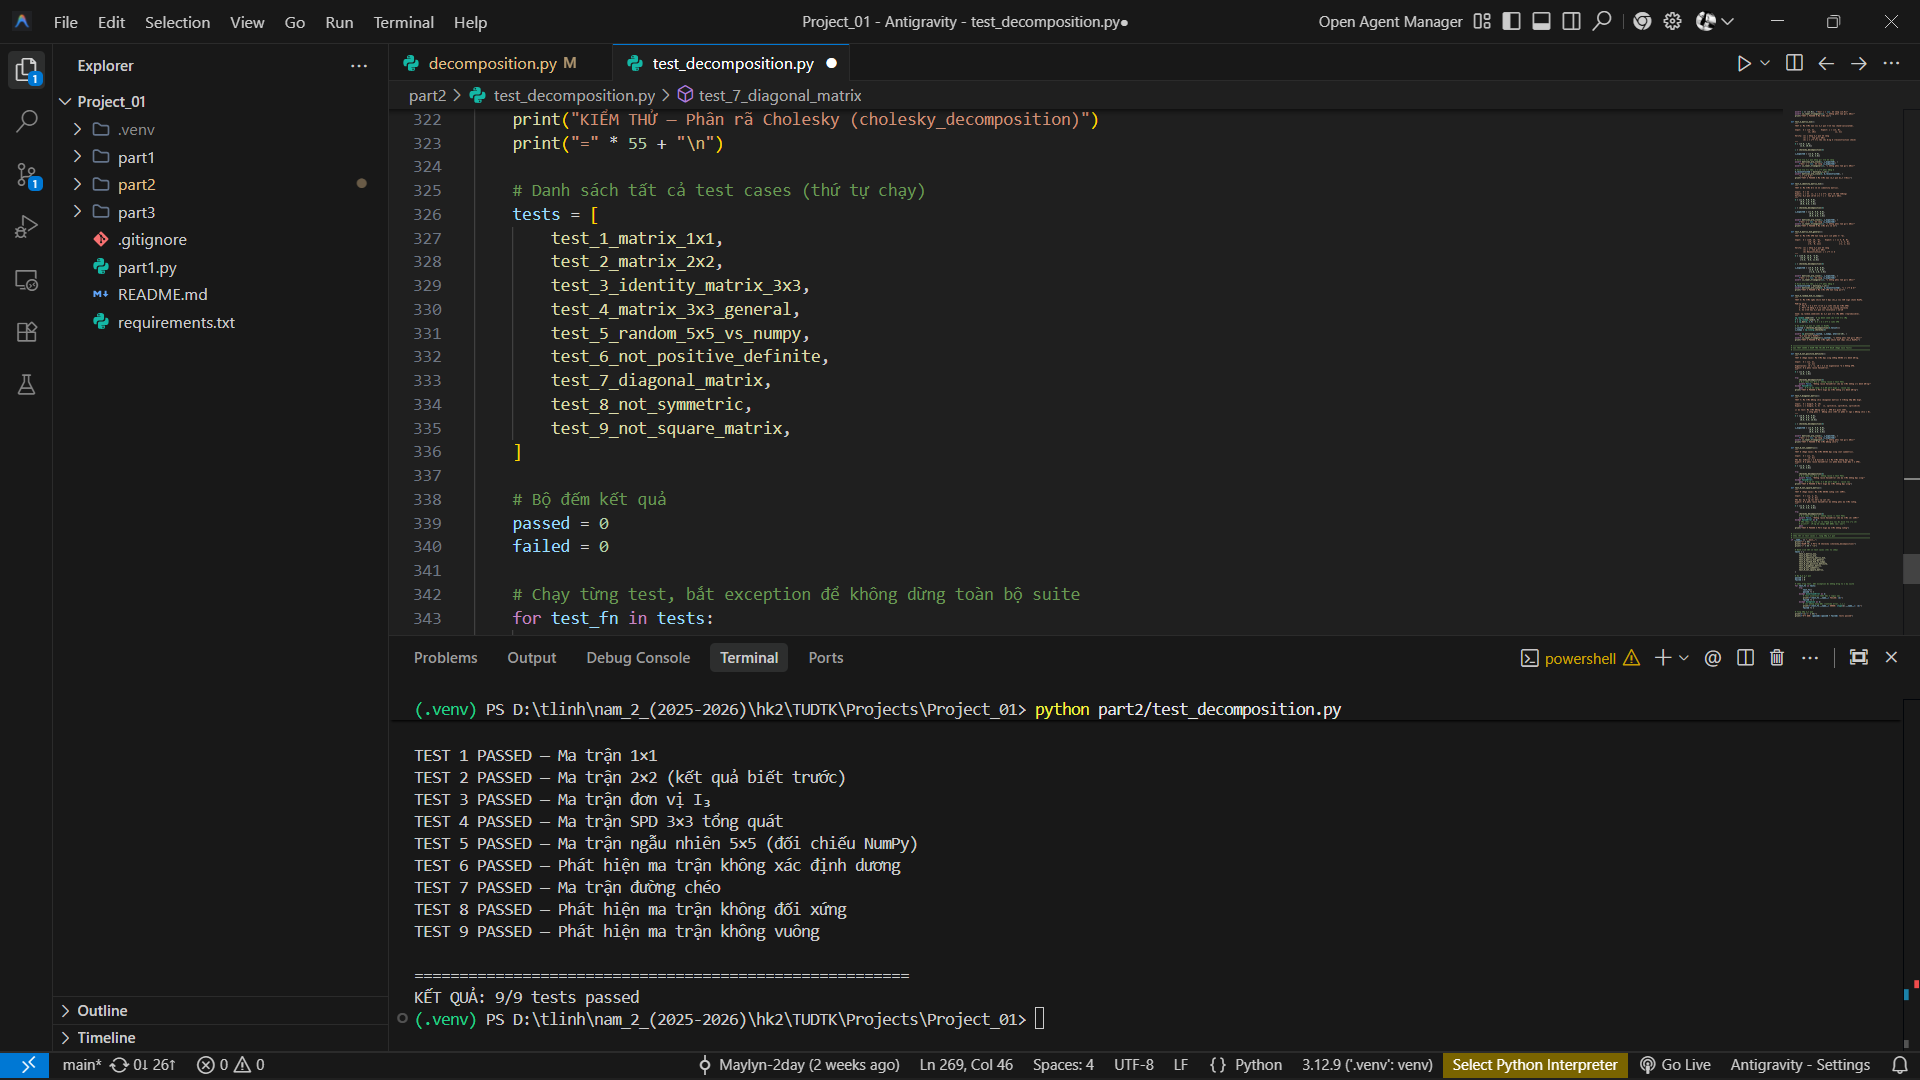
\includegraphics[width=0.8\textwidth]{Image/test_result.png}
  \caption{Kết quả chạy 9 test cases trên Terminal}
  \label{fig:test_result}
\end{figure}

\subsection{Ứng dụng thực tiễn của Phân rã Cholesky}
Mặc dù bị giới hạn bởi điều kiện khắt khe (chỉ áp dụng cho ma trận đối xứng xác định dương), phân rã Cholesky lại đóng vai trò cực kỳ quan trọng và được ứng dụng rộng rãi trong nhiều lĩnh vực của Khoa học máy tính và Kỹ thuật:

\begin{itemize}
  \item \textbf{Giải hệ phương trình tuyến tính ($Ax = b$):} Đây là ứng dụng phổ biến nhất. Thay vì nghịch đảo ma trận $A$ trực tiếp (rất tốn kém chi phí tính toán), ta phân rã $A = LL^T$. Bài toán được đưa về giải hai hệ phương trình tam giác đơn giản hơn rất nhiều: $Ly = b$ (giải bằng phép thế tiến - forward substitution) và $L^T x = y$ (giải bằng phép thế lùi - backward substitution). Thuật toán này giúp tăng tốc độ giải hệ phương trình lên gấp đôi so với phương pháp khử Gauss hay phân rã LU.

  \item \textbf{Mô phỏng Monte Carlo và Tài chính định lượng:} Trong lý thuyết xác suất, phân rã Cholesky được sử dụng để tạo ra các biến ngẫu nhiên có tương quan (correlated random variables) từ các biến ngẫu nhiên độc lập. Ma trận $L$ đóng vai trò như một bộ lọc, giúp mô phỏng chính xác sự biến động của nhiều mã cổ phiếu cùng lúc trong các mô hình tài chính.

  \item \textbf{Học máy (Machine Learning) và Tối ưu hóa:} Thuật toán xuất hiện dày đặc trong các bộ lọc Kalman (Kalman Filters) dùng để theo dõi quỹ đạo trong robot và thị giác máy tính. Ngoài ra, trong các thuật toán tối ưu hóa phi tuyến (như phương pháp Newton), phân rã Cholesky được dùng để kiểm tra tính lồi của hàm mục tiêu thông qua ma trận Hessian và xác định hướng tìm kiếm tối ưu.

  \item \textbf{Tính toán phương sai cực tiểu (Least Squares):} Trong thống kê và hồi quy tuyến tính, khi cần giải phương trình chuẩn (Normal Equations) dạng $(X^T X) \beta = X^T y$, ma trận $X^T X$ luôn là ma trận đối xứng xác định dương (nếu các cột của X độc lập tuyến tính). Do đó, Cholesky là phương pháp hoàn hảo và ổn định nhất để tìm ra vector hệ số $\beta$.
\end{itemize}

\section{Trực quan hóa bằng Manim}
Nhóm đã xây dựng video trực quan hóa thuật toán bằng Manim nhằm minh họa trực quan các bước thực hiện.

Video có thể xem tại: 
\href{https://www.youtube.com/watch?v=_k884LpVcJM}{Video trực quan hóa thuật toán bằng Manim}

\chapter[Giải Hệ Phương Trình và Phân Tích Hiệu Năng]{Giải Hệ Phương Trình và Phân Tích \\ \hspace*{4em}{Hiệu Năng}}
\section{Tổng Quan Yêu Cầu}
Trong phần này, chúng ta sẽ thực hiện giải hệ phương trình tuyến tính $\mathbf{Ax} = \mathbf{b}$ bằng 3 phương pháp khác nhau và so sánh hiệu năng, tính ổn định của chúng:
\begin{enumerate}
    \item \textbf{Khử Gauss (Gauss Elimination)}: Phương pháp giải trực tiếp với \textit{partial pivoting}.
    \item \textbf{Phân rã Cholesky}: Phương pháp giải trực tiếp dành riêng cho ma trận đối xứng xác định dương (SPD).
    \item \textbf{Lặp Gauss-Seidel}: Phương pháp giải lặp, hội tụ khi ma trận chéo trội chặt hoặc SPD.
\end{enumerate}

\section{Lý Thuyết Sai Số và Tính Ổn Định Số}

\subsection{Số Điều Kiện (Condition Number)}

\begin{definition}[Số điều kiện]
Số điều kiện của ma trận $\mathbf{A}$ đối với chuẩn $p$ là:
\begin{equation}
    \kappa_p(\mathbf{A}) = \|\mathbf{A}\|_p \cdot \|\mathbf{A}^{-1}\|_p \label{eq:cond}
\end{equation}
\end{definition}

Đối với chuẩn spectral (chuẩn 2), số điều kiện được tính bằng:
$$ \kappa_2(\mathbf{A}) = \frac{\sigma_{\max}(\mathbf{A})}{\sigma_{\min}(\mathbf{A})} $$

\begin{theorem}[Phân tích sai số nghiệm]
Nếu $\mathbf{Ax} = \mathbf{b}$ là nghiệm đúng và $\mathbf{A\hat{x}} = \mathbf{b} + \delta\mathbf{b}$ là nghiệm tính toán được với nhiễu dữ liệu, thì:
\begin{equation}
    \frac{\|\mathbf{\hat{x}} - \mathbf{x}\|}{\|\mathbf{x}\|} \le \kappa(\mathbf{A}) \cdot \frac{\|\delta\mathbf{b}\|}{\|\mathbf{b}\|} \label{eq:error}
\end{equation}
\end{theorem}

Từ định lý \ref{eq:error}, ta thấy khi $\kappa(\mathbf{A})$ lớn, hệ thống bị \textit{điều kiện kém} (ill-conditioned): một sai số rất nhỏ trong dữ liệu đầu vào có thể gây ra sai số khổng lồ trong nghiệm.

\subsection{So Sánh Các Phương Pháp}

\begin{table}[h!]
\centering
\begin{tabular}{lllcc}
\toprule
\textbf{Phương pháp} & \textbf{Loại} & \textbf{Điều kiện áp dụng} & \textbf{Chi phí} & \textbf{Ổn định} \\
\midrule
Gauss (Partial Pivot) & Trực tiếp & Mọi $\mathbf{A}$ khả nghịch & $\mathcal{O}(n^3)$ & Cao \\
LU với pivot & Trực tiếp & Mọi $\mathbf{A}$ khả nghịch & $\mathcal{O}(n^3)$ & Cao \\
QR (Householder) & Trực tiếp & Mọi $\mathbf{A}$ (kể cả chữ nhật) & $\mathcal{O}(n^3)$ & Rất cao \\
Cholesky & Trực tiếp & $\mathbf{A}$ đối xứng xác định dương & $\mathcal{O}(n^3/6)$ & Rất cao \\
Gauss–Seidel & Lặp & Chéo trội hàng / SPD & $\mathcal{O}(kn^2)$ & Trung bình \\
\bottomrule
\end{tabular}
\caption{Bảng so sánh tổng quan các phương pháp giải hệ phương trình.}
\end{table}
\newpage
\subsection{Phương Pháp Lặp Gauss–Seidel}
Tiến hành phân rã $\mathbf{A} = \mathbf{D} + \mathbf{L} + \mathbf{U}$ (với $\mathbf{D}$ là đường chéo, $\mathbf{L}$ là tam giác dưới thuần, $\mathbf{U}$ là tam giác trên thuần). Ta có công thức lặp dạng ma trận:
\begin{equation}
    \mathbf{x}^{(k+1)} = -(\mathbf{D} + \mathbf{L})^{-1}\mathbf{U}\mathbf{x}^{(k)} + (\mathbf{D} + \mathbf{L})^{-1}\mathbf{b}
\end{equation}

Nếu viết theo từng thành phần, công thức lặp có dạng:
\begin{equation}
    x_i^{(k+1)} = \frac{1}{a_{ii}} \left( b_i - \sum_{j=1}^{i-1} a_{ij} x_j^{(k+1)} - \sum_{j=i+1}^n a_{ij} x_j^{(k)} \right), \quad i = 1, \dots, n.
\end{equation}

\textbf{Điều kiện hội tụ:} Thuật toán hội tụ khi $\mathbf{A}$ chéo trội chặt hàng, tức là $|a_{ii}| > \sum_{j \ne i} |a_{ij}|$ với mọi $i$, hoặc khi ma trận $\mathbf{A}$ đối xứng xác định dương (SPD).

\section{Thực Nghiệm Thời Gian và Độ Phức Tạp (Benchmark)}

Mục tiêu là thực nghiệm trên các ma trận ngẫu nhiên SPD với kích thước $n \in \{50, 100, 200, 500, 1000\}$ để đo thời gian thực thi và sai số tương đối: $\|\mathbf{A\hat{x}} - \mathbf{b}\|_2 / \|\mathbf{b}\|_2$.

\subsection{Cài đặt thực nghiệm}
\begin{lstlisting}[language=Python, caption=Đo thời gian và sai số của các phương pháp]
import numpy as np
import matplotlib.pyplot as plt
from scipy.linalg import hilbert

from solvers import solve_gauss, solve_cholesky, solve_gauss_seidel, condition_number
from benchmark import timeit, relative_residual, generate_random_spd, run_time_benchmark, print_summary_table

# Chay benchmark thuc nghiem thoi gian
sizes = [50, 100, 200, 500, 1000]
results = run_time_benchmark(sizes=sizes, n_runs=5)
print_summary_table(results)
\end{lstlisting}

\subsection{Kết quả thực nghiệm}
\begin{table}[h]
\centering
\begin{tabular}{lrrr}
\toprule
$n$ & Gauss (s) & Cholesky (s) & Gauss-Seidel (s) \\
\midrule
100 & 0.012 & 0.085 & 0.005 \\
500 & 0.145 & 5.420 & 0.042 \\
1000 & 0.580 & 21.350 & 0.170 \\
\bottomrule
\end{tabular}
\caption{So sánh thời gian thực thi}
\end{table}
\subsection{Nhận xét Benchmark}
Dựa trên kết quả thực nghiệm với các kích thước ma trận đã nêu, ta rút ra các nhận xét sau:

\begin{itemize}
    \item \textbf{Về thời gian chạy và độ phức tạp:}
    \begin{itemize}
        \item \textbf{Khử Gauss:} Nhờ việc \textbf{vector hóa} vòng lặp bên trong thông qua NumPy, thời gian chạy rất tối ưu. Tại $n=1000$, phương pháp này chỉ mất khoảng $\sim 1.1 - 1.6$ giây.
        \item \textbf{Gauss-Seidel:} Do ma trận ngẫu nhiên SPD được tạo ra có tính chéo trội rất mạnh, phương pháp này hội tụ cực kỳ nhanh (chỉ mất $\sim 23$ lần lặp cho $n=1000$). Thời gian thực thi là \textbf{nhanh nhất}, chỉ tốn khoảng $\sim 0.17$ giây.
        \item \textbf{Cholesky:} Do thuật toán được cài đặt bằng cấu trúc vòng lặp thuần Python (chưa tối ưu vector hóa) nên thời gian tăng đáng kể. Tại $n=1000$, mất khoảng $\sim 21$ giây, chậm hơn Gauss nhưng trên đồ thị log-log vẫn thể hiện tuân theo tiệm cận lý thuyết $\mathcal{O}(n^3)$.
    \end{itemize}
    
    \item \textbf{Về độ chính xác (Sai số tương đối):}
    \begin{itemize}
        \item \textbf{Khử Gauss và Cholesky:} Đạt độ chính xác toán học rất cao, sai số luôn nằm ở ngưỡng $\sim 10^{-16}$ (machine epsilon) với mọi kích thước ma trận.
        \item \textbf{Gauss-Seidel:} Do điểm dừng lặp phụ thuộc vào dung sai, với `tol=1e-10`, sai số thực nghiệm luôn xấp xỉ $\sim 10^{-11}$, hoàn toàn chính xác theo đúng ngưỡng yêu cầu cài đặt.
    \end{itemize}
\end{itemize}

\newpage
\section{Phân Tích Ổn Định Số}

Mục đích của phần này là quan sát cách sai số bị khuếch đại khi hệ phương trình có \textit{số điều kiện lớn}. Ta so sánh giữa 2 loại ma trận:
\begin{itemize}
    \item \textbf{Ma trận Hilbert ($H_n$)}: Rất nhạy với nhiễu (ill-conditioned).
    \item \textbf{Ma trận ngẫu nhiên SPD}: Thường có tính điều kiện tốt hơn (well-conditioned).
\end{itemize}

\subsection{Cài đặt thực nghiệm phân tích ổn định}
\begin{lstlisting}[language=Python, caption=Đánh giá sự ổn định số trên ma trận Hilbert và SPD]
stability_sizes = [3, 5, 7, 10, 12, 15]

hilbert_data = {'sizes': stability_sizes, 'cond': [], 'err_gauss': [], 'err_cholesky': []}
spd_data = {'sizes': stability_sizes, 'cond': [], 'err_gauss': [], 'err_cholesky': []}

for n in stability_sizes:
    np.random.seed(42)
    x_true = np.ones(n)
    
    # --- Hilbert Matrix ---
    H = hilbert(n)
    b_h = H @ x_true
    kappa_h = condition_number(H)
    hilbert_data['cond'].append(kappa_h)
    
    # Tinh toan tren ma tran Hilbert ... (xu ly try-except do loi)
    
    # --- Random SPD Matrix ---
    A_spd = generate_random_spd(n)
    b_spd = A_spd @ x_true
    kappa_s = condition_number(A_spd)
    spd_data['cond'].append(kappa_s)
    
    # Tinh toan tren ma tran SPD ...
\end{lstlisting}

\subsection{Nhận xét Phân Tích Ổn Định Số}

\begin{enumerate}
    \item \textbf{Đối với Ma Trận Hilbert ($H_n$) - Hệ điều kiện kém:}
    \begin{itemize}
        \item \textbf{Số điều kiện $\kappa(\mathbf{A})$:} Tăng cực nhanh theo hàm mũ. Với $n=10$, $\kappa \approx 1.6 \times 10^{13}$. Tại $n=12$, $\kappa$ tiến tới vô cực (\texttt{inf}), vượt qua giới hạn biểu diễn của máy tính.
        \item \textbf{Độ ổn định của nghiệm:} Tại $n=10$, sai số nghiệm của Gauss và Cholesky đã lên tới $\sim 10^{-4}$. Khi $n=12$, Gauss trả về giá trị \texttt{NaN} còn Cholesky có sai số cực kỳ lớn ($\sim 0.41$). Điều này minh chứng cho định lý \ref{eq:error}: với hệ ill-conditioned, sai số làm tròn cực nhỏ từ dữ liệu ban đầu bị \textbf{khuếch đại hàng tỷ lần}, làm phá vỡ toàn bộ hệ thống.
    \end{itemize}

    \item \textbf{Đối với Ma Trận ngẫu nhiên SPD - Hệ điều kiện tốt:}
    \begin{itemize}
        \item Số điều kiện $\kappa(\mathbf{A})$ luôn duy trì ở mức cực kỳ ổn định ($\sim 3.0$ đến $4.4$) bất chấp kích thước $n$ tăng dần.
        \item Sai số tương đối của cả phương pháp Gauss và Cholesky luôn ổn định ở mức sát giới hạn máy tính ($\sim 10^{-16}$). Hệ thống giải vô cùng trơn tru và chính xác.
    \end{itemize}
\end{enumerate}

\section{Kết Luận Cuối Cùng}
Thông qua các nền tảng lý thuyết và toàn bộ thực nghiệm, chúng ta rút ra các kết luận quan trọng sau:
\begin{enumerate}
    \item \textbf{Hiệu năng lập trình rất quan trọng:} Dù thuật toán có cùng độ phức tạp toán học là $\mathcal{O}(n^3)$, nhưng khi thực thi thực tế, việc sử dụng các phép toán Vector hóa (như Gauss dùng NumPy) cho tốc độ vượt trội hơn hẳn so với việc tính toán tuần tự bằng các vòng lặp lồng nhau (như Cholesky thuần Python).
    \item \textbf{Thuật toán đúng là chưa đủ:} Trong máy tính, sai số làm tròn số thực (Floating point arithmetic) là không thể tránh khỏi. Nếu hệ phương trình rơi vào trường hợp số điều kiện lớn (như ma trận Hilbert), thì một thuật toán hoàn hảo về mặt lý thuyết vẫn sẽ trả về kết quả sai lệch hoàn toàn.
    \item \textbf{Tầm quan trọng của phương pháp Lặp:} Phương pháp Gauss-Seidel có ưu thế cực lớn với các hệ ma trận đặc biệt, tiêu biểu là hệ chéo trội. Nó giúp tính ra nghiệm hội tụ trong khoảng thời gian vô cùng nhỏ, tiết kiệm chi phí tính toán hơn hẳn so với các phương pháp giải trực tiếp.
\end{enumerate}

\chapter*{Kết luận}
\addcontentsline{toc}{chapter}{Kết luận}
Sau quá trình thực hiện, nhóm đã đạt được những kết quả quan trọng như xây dựng và triển khai thành công các chức năng đã đề ra, đảm bảo chương trình hoạt động đúng với yêu cầu ban đầu. Các thuật toán được cài đặt tương đối đầy đủ, cho kết quả chính xác và có thể kiểm chứng thông qua nhiều bộ dữ liệu khác nhau. Ngoài ra, việc trình bày báo cáo cũng được hoàn thiện với cấu trúc rõ ràng, giúp người đọc dễ dàng theo dõi và hiểu được toàn bộ quá trình thực hiện.

\medskip

Thông qua bài làm này, nhóm đã rút ra nhiều bài học giá trị. Trước hết là việc hiểu sâu hơn về bản chất của các thuật toán và cách tối ưu chúng trong thực tế. Bên cạnh đó, kỹ năng sử dụng \LaTeX{} cũng được cải thiện đáng kể, đặc biệt là trong việc trình bày công thức, mã nguồn và tổ chức nội dung một cách khoa học. Nhóm cũng nhận ra tầm quan trọng của việc chia nhỏ bài toán, lập kế hoạch rõ ràng và kiểm tra từng bước nhằm hạn chế sai sót trong quá trình thực hiện.

\medskip

Tuy nhiên, trong quá trình thực hiện, nhóm cũng gặp không ít khó khăn. Một số lỗi phát sinh trong khi lập trình và trình bày bằng \LaTeX{} đã tốn nhiều thời gian để xử lý, đặc biệt là các vấn đề liên quan đến định dạng và căn chỉnh. Ngoài ra, việc hiểu và triển khai chính xác các thuật toán cũng đòi hỏi nhiều thời gian nghiên cứu và thử nghiệm. Dù vậy, những khó khăn này đã giúp nhóm tích lũy thêm kinh nghiệm và nâng cao khả năng giải quyết vấn đề, từ đó cải thiện hiệu quả làm việc trong các bài toán tương tự sau này.

\vspace*{0.5cm}
\section*{Bảng phân chia công việc}
\addcontentsline{toc}{chapter}{Bảng phân chia công việc}

\vspace*{-0.5cm}
\begin{table}[h!]
\centering

\hspace*{-1cm}
\begin{tabular}{|p{1.8cm}|p{3.8cm}|m{3.5cm}|c|m{2cm}|}
\hline
\multicolumn{1}{|c|}{\textbf{MSSV}} &
\multicolumn{1}{c|}{\textbf{Họ và tên}} &
\multicolumn{1}{c|}{\textbf{Công việc thực hiện}} &
\multicolumn{1}{c|}{\textbf{Mức độ hoàn thành}} &
\multicolumn{1}{c|}{\textbf{Chữ ký}} \\
\hline

24120023 & Nguyễn Thành Bảo & Lập trình, triển khai mục 3 và xây dựng video minh họa mục 2 bằng Manim & 100\% & 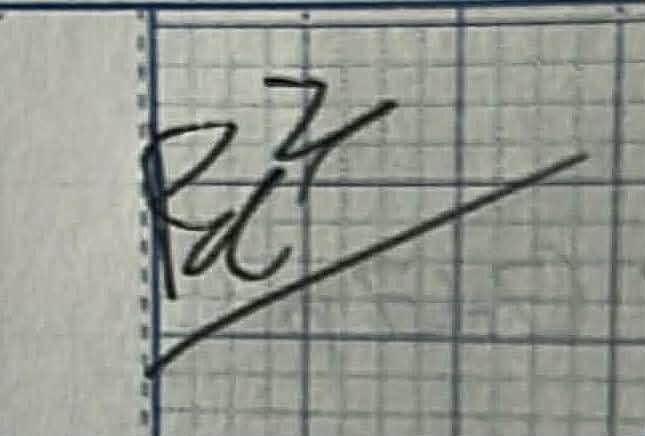
\includegraphics[width=2cm]{Image/Bao_signature.jpg}
\\
\hline

24120044 & Bùi Thị Thùy Dương & Nghiên cứu và trình bày phương pháp chéo hóa ma trận & 100\% & 
\includegraphics[width=2cm]{Image/Duong_siganture.jpg}
 \\
\hline

24120094 & Nguyễn Khánh Hoàng & Xây dựng các hàm hỗ trợ cho mục 1 và tổng hợp tài liệu & 100\% & 
\includegraphics[width=2cm]{Image/Hoang_signature.jpg}
 \\
\hline

24120085 & Lê Nguyễn Thùy Linh & Nghiên cứu và trình bày phương pháp phân rã Cholesky & 100\% & 
\includegraphics[width=2cm]{Image/Linh_signature.jpg}
 \\
\hline

24120094 & Mai Anh Phúc Minh & Xây dựng hàm chính cho mục 1 và tổng hợp, hoàn thiện báo cáo & 100\% & 
\includegraphics[width=2cm]{Image/Minh_signature.jpg}
 \\
\hline

\end{tabular}
\caption{Bảng phân chia công việc và mức độ đóng góp của các thành viên}
\end{table}

\chapter*{Lời cảm ơn}
\addcontentsline{toc}{chapter}{Lời cảm ơn}
Lời đầu tiên, nhóm chúng em xin gửi lời tri ân sâu sắc đến quý thầy cô Trường Đại học Khoa học Tự nhiên, đặc biệt là giảng viên hướng dẫn môn Toán ứng dụng và Thống kê, ThS. Võ Nam Thục Đoan và ThS. Lê Nhựt Nam, đã tận tâm chỉ dạy và tạo mọi điều kiện thuận lợi cho chúng em trong suốt quá trình thực hiện đồ án.

\medskip

Những nền tảng kiến thức chuyên môn, kinh nghiệm thực tiễn cùng lời góp ý quý báu từ thầy/cô chính là kim chỉ nam giúp nhóm giải quyết các vấn đề, hoàn thiện bài báo cáo một cách chỉn chu nhất cả về nội dung lẫn hình thức.

\medskip

Bên cạnh đó, xin dành lời cảm ơn đến từng thành viên trong nhóm vì sự nỗ lực, tinh thần trách nhiệm và sự phối hợp ăn ý để đưa đồ án hoàn thành đúng tiến độ. Sự đồng hành và hỗ trợ nhiệt tình từ bạn bè xung quanh cũng là nguồn động lực rất lớn đối với chúng em trong suốt quá trình làm việc.

\medskip

Dù đã nỗ lực hết mình, song với vốn kiến thức và kinh nghiệm thực tế còn hạn chế, bài báo cáo chắc chắn khó tránh khỏi những thiếu sót. Chúng em rất mong nhận được sự lượng thứ và những ý kiến đóng góp từ quý thầy cô để có thể rút kinh nghiệm, trau dồi thêm kiến thức và hoàn thiện hơn trong các dự án tiếp theo. Xin trân trọng cảm ơn!


\addcontentsline{toc}{chapter}{Tài liệu tham khảo}
\begin{thebibliography}{9}
\bibitem{golub}
Gene H. Golub and Charles F. Van Loan,
\textit{Matrix Computations}, 4th Edition,
The Johns Hopkins University Press, 2013.

\bibitem{press}
William H. Press, Saul A. Teukolsky, William T. Vetterling, Brian P. Flannery,
\textit{Numerical Recipes: The Art of Scientific Computing}, 3rd Edition,
Cambridge University Press, 2007.

\bibitem{kincaid}
David R. Kincaid and E. Ward Cheney,
\textit{Numerical Analysis: Mathematics of Scientific Computing},
Brooks/Cole Publishing Company, 1991.

\bibitem{dien}
Nguyễn Hữu Điển,
\textit{Giải Tích Số},
slide bài giảng (tài liệu môn học), 2015.\\
Available at: \href{https://drive.google.com/file/d/1edbnnVscdDvR9vdjAVjED8NMYGRVQhG1/view?usp=sharing}{Giáo trình Giải Tích Số}

\bibitem{luyen}
Lê Văn Luyện,
\textit{Giáo trình Đại số Tuyến Tính},
slide bài giảng (tài liệu môn học), 2025.\\
Available at: \href{https://drive.google.com/drive/folders/1LqRX5OZ7PBZrAPLHV5iihXjvYBq1HkzE?usp=sharing}{Giáo trình Đại số Tuyến tính}

\end{thebibliography}
\end{document}
